%%%%%%%%%%%%%%%%%%%%%%%%%%%%%%%%%%%%%%%%%
% University/School Laboratory Report
% LaTeX Template
% Version 3.1 (25/3/14)
%
% This template has been downloaded from:
% http://www.LaTeXTemplates.com
%
% Original author:
% Linux and Unix Users Group at Virginia Tech Wiki 
% (https://vtluug.org/wiki/Example_LaTeX_chem_lab_report)
%
% License:
% CC BY-NC-SA 3.0 (http://creativecommons.org/licenses/by-nc-sa/3.0/)
%
%%%%%%%%%%%%%%%%%%%%%%%%%%%%%%%%%%%%%%%%%

%----------------------------------------------------------------------------------------
%	PACKAGES AND DOCUMENT CONFIGURATIONS
%----------------------------------------------------------------------------------------

\documentclass{article}
\usepackage[spanish,es-tabla]{babel}
\newcommand\Monthname[1][EMPTY]{%
  \ifnum1=#1Enero\else
  \ifnum2=#1Febrero\else
  \ifnum3=#1Marzo\else
  \ifnum4=#1Abril\else
  \ifnum5=#1Mayo\else
  \ifnum6=#1Junio\else
  \ifnum7=#1Julio\else
  \ifnum8=#1Agosto\else
  \ifnum9=#1Septiembre\else
  \ifnum10=#1Octubre\else
  \ifnum11=#1Noviembre\else
  \ifnum12=#1Diciembre\else
  \fi\fi\fi\fi\fi\fi\fi\fi\fi\fi\fi\fi
}

\usepackage{datetime}

\usepackage[a4paper,
 %left=20mm,
 top=30mm,
 bottom=25mm,
 headheight=80pt,
 headsep=15mm
 ]{geometry}


\usepackage[version=3]{mhchem} % Package for chemical equation typesetting
\usepackage{graphicx} % Required for the inclusion of images

\usepackage{amsfonts}
\usepackage{amsmath} % Required for some math elements 
\usepackage{mathtools}

\usepackage{multirow}

\DeclarePairedDelimiter{\ceil}{\lceil}{\rceil} %this is for ceil and floor symbols
\DeclarePairedDelimiter{\floor}{\lfloor}{\rfloor} %this is for ceil and floor symbols

\usepackage{changepage} % Required in text margins
\usepackage{xcolor} % Required changing color 
\usepackage{sectsty} %Required to change section headers
\usepackage{titlesec} % Required for section spacing
\usepackage{enumitem}
\usepackage{tocloft} % Better in table of contents
\usepackage[blocks]{authblk}% The option is for block layout
\usepackage[pdfborder={0 0 0}]{hyperref}% For email addresses
\usepackage{fancyhdr} %Required for Headers

\usepackage[nottoc]{tocbibind} %Better to add references and more in table of contents (nottoc is to remove indice in toc)

\usepackage{layout} %Used for "margin debugging"

\usepackage[export]{adjustbox} 
\usepackage{float}

\usepackage{subfig}% http://ctan.org/pkg/subfig

\usepackage{lineno} %required to line number
\linenumbers

\usepackage{tikz} %required to schemes
\usetikzlibrary{mindmap}


\pagestyle{fancy}
\fancyheadoffset{0cm} %Used for heading without margins
\fancyhead[L]{} % 1. sectionname

\rhead{ \textit{Simulaci\'on y Animaci\'on Biomec\'anica de un Humanoide}}
\renewcommand{\headrulewidth}{0.4pt}


\renewcommand\cfttoctitlefont{\hfill\huge\bfseries\color{cyan}}
\renewcommand\cftaftertoctitle{\hfill\mbox{}}

\setlist{leftmargin=5.5mm}

\titlespacing*{\section} {0pt}{6ex}{2ex}
\titlespacing*{\subsection} {0pt}{4ex}{0.7ex}

\sectionfont{\color{cyan}} % Changing color to section headers
\subsectionfont{\color{cyan}} % Changing color to subsection headers
\subsubsectionfont{\color{cyan}} % Changing color to subsubsection headers
\paragraphfont{\color{cyan}} % Changing color to subsubsubsection headers
%\setlength\parindent{0pt} % Removes all indentation from paragraphs

\renewcommand{\labelitemi}{$-$}

\renewcommand{\baselinestretch}{1.25} 

\renewcommand{\labelenumi}{\alph{enumi}.} % Make numbering in the enumerate environment by letter rather than number (e.g. section 6)

\let\datespanish\relax
\newdateformat{datespanish}{\Monthname[\THEMONTH] \THEYEAR}

\setcounter{secnumdepth}{4} % Enabling subsubsubsections (in \paragraph keyword)
\setcounter{tocdepth}{4} % Table of contents with level 4


\usepackage{etoolbox}
\apptocmd{\thebibliography}{\leftmargin\labelwidth}{\leftmargin\labelwidth\labelsep=10pt}{}{}


%\usepackage{times} % Uncomment to use the Times New Roman font

%----------------------------------------------------------------------------------------
%	DOCUMENT INFORMATION
%----------------------------------------------------------------------------------------

\title{\textbf{\Large{\\ \underline{PROYECTO} \underline{FINAL} \\ \vspace*{2ex} INGENIER\'IA INFORM\'ATICA - ITBA \\}} \vspace*{4ex} 
\textbf{\textcolor{cyan}{\textit{SIMULACI\'ON Y ANIMACI\'ON BIOMEC\'ANICA \\DE UN HUMANOIDE}  }  \vspace*{3ex}} } % Title

\author{\textbf{Alumnos:} }
\affil{\textbf{Enzo Altamiranda Graterol}\\% If the blocks option of authblk is removed \\ is treated as ,
\url{ealtamir@itba.edu.ar}}

\affil{\textbf{Teresa Fontanella De Santis}\\
\url{tfontane@itba.edu.ar}}

\affil{\textbf{Tom\'as Mehdi}\\
\url{tmehdi@itba.edu.ar}\vspace*{3ex}}

\author{\textbf{Tutor:}}
\affil{ \textbf{Dr. Daniel Ricardo Parisi} \vspace*{8ex}}

\date{\textbf{\small{\today}}} % Date for the report

\author{  \small{\textbf{Instituto Tecnol\'ogico de Buenos Aires - ITBA \\  Departamento de Ingenier\'ia Inform\'atica} }  }
\affil{\vspace*{0ex}}

\tikzset{
  every picture/.append style={
  execute at begin picture={\deactivatequoting},
  execute at end picture={\activatequoting}
  }
}


\begin{document}

% \layout %CAREFUL!! This is only for "debugging"

\maketitle % Insert the title, author and date
\thispagestyle{empty} %Page without number

\newpage
\tableofcontents
\newpage

% If you wish to include an abstract, uncomment the lines below
 \begin{abstract}
 
\addcontentsline{toc}{section}{Resumen} %Including abstract in table of contents
\noindent

\begin{adjustwidth}{1.05cm}{0cm}
Este proyecto tiene como objetivo crear una simulaci\'on y animaci\'on de un humano virtual, con las siguientes propiedades:
\begin{itemize}[leftmargin=5.5mm]
\item Biomec\'anica: que tanto su estructura (peso, altura y posici\'on de cada una de sus partes) como su interacci\'on con el entorno, respondan a comportamientos f\'isicos reales y exactos.
\item Inteligencia artificial: que aprenda a caminar por s\'i mismo, utilizando para ello m\'etodos de \textit{soft computing} como algoritmos gen\'eticos.
\end{itemize}

\end{adjustwidth}

 \end{abstract}

%(---------------------------------------------------------------------------------------
%	SECTION 1 - INTRODUCCION
%----------------------------------------------------------------------------------------


\section{Introducci\'on}

%\begin{adjustwidth}{1cm}{0cm}
Siempre ha sido de inter\'es la simulaci\'on biomec\'anica de seres vivos, especialmente en las ciencias naturales (zoolog\'ia, medicina, etc.). \\
Ahora bien, \'ultimamente se ha incrementado el inter\'es en otras \'areas de aplicaci\'on, como los videojuegos (creaci\'on de personajes con reacciones m\'as reales), y la ingenier\'ia (verbigracia: dise\~no de espacios cerrados, con mayores medidas de seguridad).\\
Una caracter\'istica muy importante de este trabajo es que el humanoide no es fruto de una animaci\'on realizada por un artesano, que mueve cada uno de los segmentos a mano; sino un objeto compuesto de segmentos f\'isicos, que interaccionan entre s\'i y con el entorno por medio de las leyes f\'isicas; agregando as\'i realismo a la situaci\'on simulada.  La otra propiedad es que el b\'ipedo aprenda por s\'i solo a caminar en l\'inea recta, sin tener en su trayectoria ning\'un obst\'aculo.\\
Este problema se puede abordar de diversas maneras, involucrando: redes neuronales\footnote{Una red neuronal es un paradigma de aprendizaje autom\'atico. Se trata de un sistema de interconexi\'on de neuronas que colaboran entre s\'i, para producir un est\'imulo de salida. Dada una entrada del sistema, se produce una salida, originada por varias transformaciones intermedias.}, sistemas de control\footnote{Un sistema de control es un dispositivo (o conjunto de) que maneja, dirige o regula el comportamiento de otros dispositivos o sistemas, para minimizar los fallos y obtener los resultados deseados.} (\textit{passive walkers}\footnote{Un \textit{passive walker} utiliza el movimiento natural (\textit{swinging}) de las piernas para ahorrar energ\'ia usada por motores. Para caminar, calcula la posici\'on de ciertos puntos (las articulaciones, mayormente).})\cite{Wojtyra}, algoritmos gen\'eticos\footnote{Los algoritmos gen\'eticos son m\'etodos adaptativos, que pueden ser utilizados para resolver problemas de b\'usqueda y optimizaci\'on. Est\'an basados en la teor\'ia de la selecci\'on natural, planteada por Charles Robert Darwin en 1859.}\cite{flexibleMuscle}, entre otras. Varios de ellos implican modelos te\'oricos complejos de humanoide (considerando m\'usculos con distintos materiales, etc.). \\
Asimismo, existe un trabajo previo cuyo prop\'osito era lograr la caminata de un cuadr\'upedo virtual, utilizando algoritmos gen\'eticos\cite{Cuadrupedo}. Continuando con esta \'ultima l\'inea de investigaci\'on y extendi\'endola a b\'ipedos, en este proyecto tambi\'en se busc\'o aplicar algoritmos gen\'eticos, y lograr la caminata usando un modelo de humanoide basado en un conjunto de segmentos (cuerpos r\'igidos), unidos entre s\'i por articulaciones, cuyo desplazamiento depende de torques aplicados a dichos cuerpos, y sus par\'ametros se ajustan a partir de la evoluci\'on del algoritmo. \\
El presente informe, describe y analiza pormenorizadamente: en la secci\'on 2, las herramientas aplicadas; en la 3, el modelo del humanoide utilizado; en la 4 y 5, los diferentes tipos de actuadores y funciones de partida y contorno; en la 6, el algoritmo gen\'etico; y en la 7 y 8, los resultados obtenidos con sus respectivas conclusiones.

%\end{adjustwidth}

\newpage

%----------------------------------------------------------------------------------------
%	SECTION 2 - HERRAMIENTAS
%----------------------------------------------------------------------------------------

\section{Herramientas}

%\begin{adjustwidth}{1cm}{0cm}
\subsection{Motor f\'isico}

%\begin{adjustwidth}{1.2cm}{0cm}
Se llama motor f\'isico o \textit{physics engine} a un  ``\textit{software} capaz de realizar simulaciones de ciertos sistemas f\'isicos, como la din\'amica del cuerpo r\'igido, el movimiento de un fluido y la elasticidad" \cite{wikiPhysicsEngine}. \\
Actualmente, existen muchos motores f\'isicos: ya sea de c\'odigo propietario (\textit{PhysX}, \textit{Havok}), como \textit{open-source} (\textit{Bullet Physics}, \textit{Box2D}, \textit{Newton}, \textit{OGRE}). Considerando an\'alisis relacionados \cite{Comparissons}\cite{Comparissons2}, y el hecho de que el espacio simulado fuese en 3D, se decidi\'o que \textit{Bullet Physics}\cite{LinkBullet} es el m\'as id\'oneo. Est\'a implementado en C++ y ha sido utilizado en varios juegos (\textit{Grand Theft Auto IV} y \textit{V}, etc); en los efectos especiales de pel\'iculas (\textit{Hancock}, \textit{Bolt}, etc.); y proyectos cient\'ificos, como la herramienta \textit{open-source} \textit{Tensegrity Robotics Toolkit} de la NASA\footnote{http://bulletphysics.org/Bullet/phpBB3/viewtopic.php?f=17\&t=9978}; entre otros.\\
Si bien (como se ver\'a m\'as adelante) \textit{Bullet} tiene problemas asociados con el coeficiente de restituci\'on, posee una muy buena \textit{performance} en la detecci\'on de colisiones, la din\'amica y la resoluci\'on de \textit{constraints}. Esto se debe, en parte, a diferentes algoritmos iterativos de orden lineal (donde el m\'as importante es \textit{Sequential Impulse}), de \textit{caching} y tambi\'en a la utilizaci\'on de un modelo de fricci\'on de Coulomb aproximado \cite{Catto}. Adem\'as, el motor f\'isico brinda la posibilidad de regular la precisi\'on requerida en estos c\'alculos (sin olvidar que, con iguales recursos, a mayor precisi\'on, mayor capacidad de c\'omputo requerida y, ergo, mayor tiempo). Dado que la construcci\'on del humanoide implica definir caracter\'isticas y restricciones de movimiento de cada uno de sus segmentos, lo antes mencionado fue crucial para la elecci\'on de \textit{Bullet Physics} en este proyecto.

\subsubsection{Funcionamiento}
El motor f\'isico se encarga de la simulaci\'on de cuerpos r\'igidos y la interacci\'on entre los mismos.
En particular debe calcular el resultado de colisiones, arreglar el solapamiento
de los cuerpos en el espacio de simulaci\'on, estimar las fuerzas producidas debido a la fricci\'on, 
y mantener el cumplimiento de restricciones que puedan existir entre los cuerpos 
(por ejemplo, un v\'inculo para formar una articulaci\'on). Para lograrlo, \textit{Bullet} modela, 
a partir de un conjunto de ecuaciones, las distintas restricciones que deben ser respetadas. \\ 
Estos modelos reciben como dato la velocidad lineal
y angular de cada objeto, y las fuerzas que act\'uan sobre los mismos. Dada esta
informaci\'on, se resuelve el sistema de ecuaciones, cuya soluci\'on representa
las magnitudes de las fuerzas a accionar sobre el mismo, a fin de satisfacer todas las
restricciones. Para encontrar esta soluci\'on, entran en juego los distintos m\'etodos de
complejidad lineal mencionados en la subsecci\'on anterior. \\
Este procedimiento, se lleva a cabo en cada \textit{timestep} de la simulaci\'on; donde un \textit{timestep}
es el intervalo de tiempo que transcurre entre un c\'alculo de magnitudes y otro. Mientras 
menor sea el \textit{timestep}, el simulador ser\'a m\'as preciso pero tambi\'en consumir\'a m\'as tiempo
de c\'omputo.



%\end{adjustwidth}
\subsubsection{Modelo de fricci\'on y su verificaci\'on}

%\begin{adjustwidth}{1.3cm}{0cm}
Hay reglas f\'isicas relacionadas con el entorno y que son muy importantes para la caminata: el modelo de fricci\'on, con sus respectivos coeficientes de fricci\'on y restituci\'on.\\  
En base a los modelos f\'isico-matem\'aticos que representan a cada uno de los dos fen\'omenos en cuesti\'on (y que se explicar\'an a continuaci\'on), y pensando en posibles futuras simulaciones de varios humanoides chocando e interactuando entre s\'i; se llevaron a cabo dos ensayos para verificar el funcionamiento del simulador f\'isico \textit{Bullet}.

\paragraph{Verificaci\'on del coeficiente de fricci\'on}\mbox{}

Para determinar el modelo utilizado por \textit{Bullet} para simular las fuerzas resultantes sobre un cuerpo por acci\'on de la fricci\'on, se simul\'o un cubo, de $m_{cube}=1kg$ y $l_{cube}=1m$, que tiene una velocidad inicial constante ($v_{i}$) en el eje horizontal, que gradualmente se detiene por acci\'on de la fricci\'on, hasta llegar al reposo (Fig. \ref{fig:translatingCube}).\\
\begin{figure}[H]%
  \centering
  \frame{\includegraphics[width=0.4\linewidth]{translatingCube.png}}
    \caption{Visualizaci\'on del sistema del cubo}
    \label{fig:translatingCube} 
\end{figure}
\noindent Para esta prueba se utiliz\'o el modelo matem\'atico que representa la posici\'on del cuerpo en el eje horizontal en funci\'on del tiempo $t$, representado por la siguiente ecuaci\'on: 
 \begin{equation}
  x(t) = x_i +v_i t+\frac{1}{2} at^2
\end{equation}
En este caso, el cuerpo empieza su movimiento en el origen, por lo tanto la posici\'on inicial ($x_i$) es cero. $v_{i}$ es la velocidad inicial, y $a$, la aceleraci\'on. Debido a la fricci\'on entre el cuerpo y el suelo, se genera una fuerza de rozamiento $\boldsymbol{ F_{\mu_{d}} } $\footnote{En las ecuaciones, los vectores se escriben en negrita.} (ec. (2)) en la misma direcci\'on que la velocidad del s\'olido y en sentido contrario.
\begin{equation}
  -\boldsymbol{ F_{\mu_d} } = \mu_d \boldsymbol{F_N} 
\end{equation}
donde $\boldsymbol{F_N}=mg$ es la fuerza normal que act\'ua sobre la caja de masa $m$ por acci\'on de la gravedad $g = 10 \frac{m}{s}$, y $\mu_d$ es el coeficiente de fricci\'on din\'amico.\\\\
Finalmente, se obtiene la aceleraci\'on:
 \begin{equation}
  a = \frac{  \boldsymbol{F_{\mu_d}}   }{m}= \frac{-\mu_d\boldsymbol{F_N}}{m} = \frac{-\mu_d mg}{m} = -\mu_dmg
\end{equation}
Considerando las ec. (1) y (3), se puede obtener el modelo matem\'atico que predice el movimiento de la caja:
 \begin{equation}
 \label{modelo_cube}
  x(t) = x_i +v_i t-\frac{1}{2} \mu_d gt^2
\end{equation}
\\
El intervalo de tiempo f\'isico (o \textit{timestep}) utilizado es $\Delta t=\frac{1}{60} s$. El \textit{timestep} de animaci\'on (es decir,
cada cu\'anto tiempo se guardan en un archivo los datos logrados) es $\Delta t' = $0.1 y el tiempo de simulaci\'on es de $s=100\Delta t$.\\
Seguidamente, se muestran los gr\'aficos obtenidos al correr los experimentos num\'ericos con los siguientes valores: $v_{i}= \{$ 1, 3 y 10$\} \frac{m}{s}$ y $\mu_{d}= \{ $0.25, 0.50 y 0.75$\} $. Se compara la distancia en el eje Z de la caja en Bullet, con su distancia en el mismo eje seg\'un la ec. (\ref{modelo_cube}). 
\begin{figure}[H]%
  \centering
  \subfloat[][]{
  	\centering
	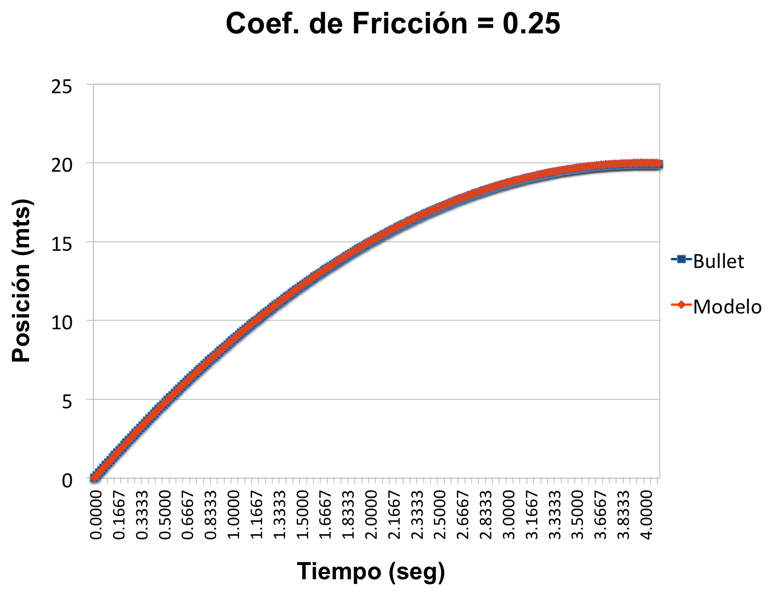
\includegraphics[width=0.6\linewidth]{image001.png} 
	\label{fig1:a} 
  }%
  \\
  \subfloat[][]{
  	\centering
	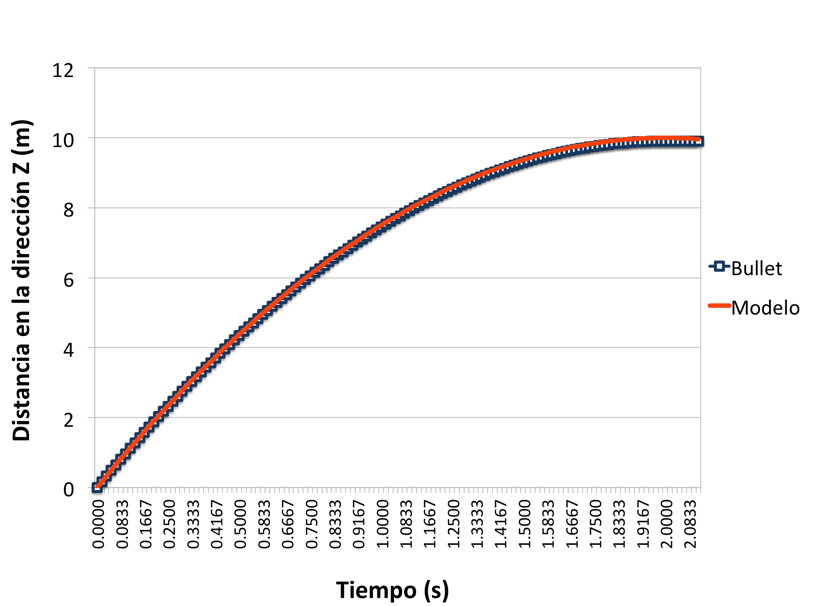
\includegraphics[width=0.6\linewidth]{image003.png} 
	\label{fig1:b} 
  }
  \\
  \subfloat[][]{
  	\centering
	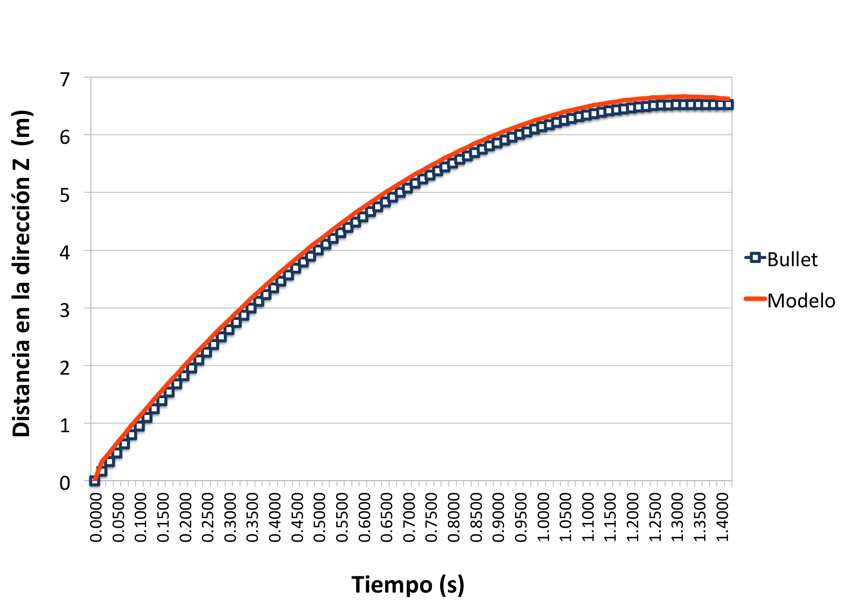
\includegraphics[width=0.6\linewidth]{image002.png} 
	\label{fig1:c} 
  }
  \captionsetup{justification=centering}
  \caption{Resultados logrados de simular el sistema descripto en Fig. \ref{fig:translatingCube}, usando $v_i = 10 \frac{m}{s}$ y: \\ (\protect\subref*{fig1:a}) $\mu_d=$0.25, (\protect\subref*{fig1:b}) $\mu_d=$0.50, y (\protect\subref*{fig1:c}) $\mu_d=$0.75}%
  \label{fig1} %
\end{figure}

\begin{figure}[H]%
  \centering
  \subfloat[][]{
  	\centering
	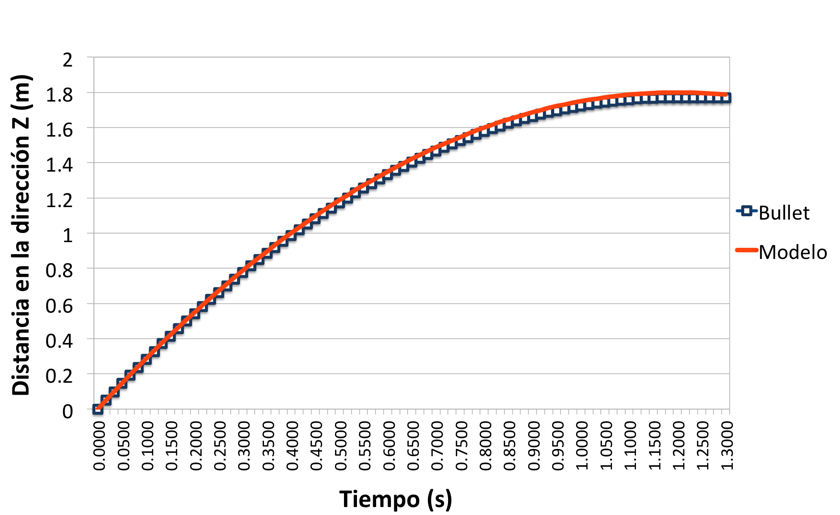
\includegraphics[width=0.6\linewidth]{image009.png} 
	\label{fig2:a} 
  }%
  \vspace*{6ex}
  \subfloat[][]{
  	\centering
	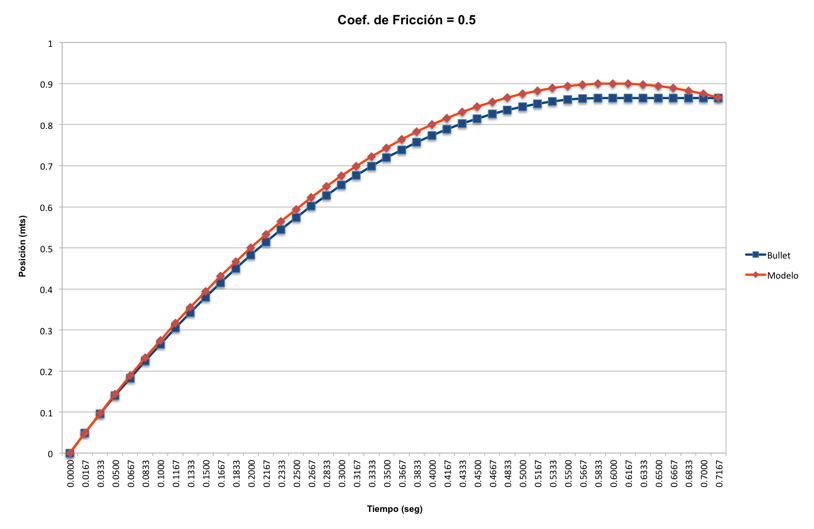
\includegraphics[width=0.6\linewidth]{image007.png} 
	\label{fig2:b} 
  }
  \vspace*{6ex}
  \subfloat[][]{
  	\centering
	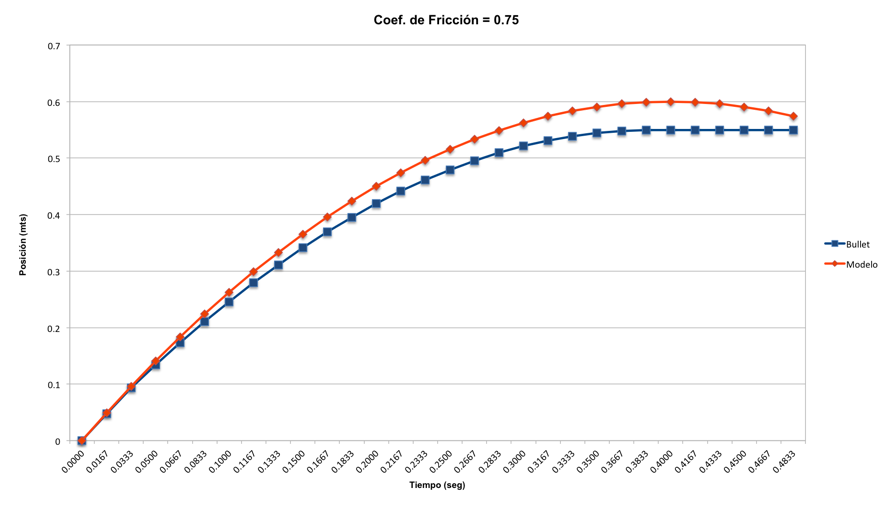
\includegraphics[width=0.6\linewidth]{image008.png} 
	\label{fig2:c} 
  }
   \captionsetup{justification=centering}
  \caption{Resultados logrados de simular el sistema descripto en Fig. \ref{fig:translatingCube}, usando $v_i = 3 \frac{m}{s}$ y:\\ (\protect\subref*{fig2:a}) $\mu_d=$0.25, (\protect\subref*{fig2:b}) $\mu_d=$0.50, y (\protect\subref*{fig2:c}) $\mu_d=$0.75}%
  \label{fig2} %
\end{figure}

\begin{figure}[H]%
  \centering
  \subfloat[][]{
  	\centering
	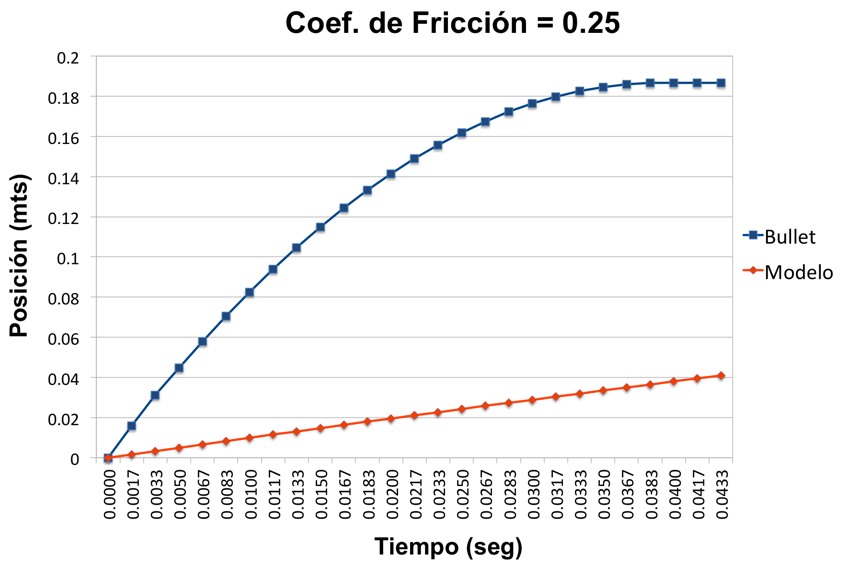
\includegraphics[width=0.6\linewidth]{image004.png} 
	\label{fig3:a} 
  }%
  \vspace*{0ex}
  \subfloat[][]{
  	\centering
	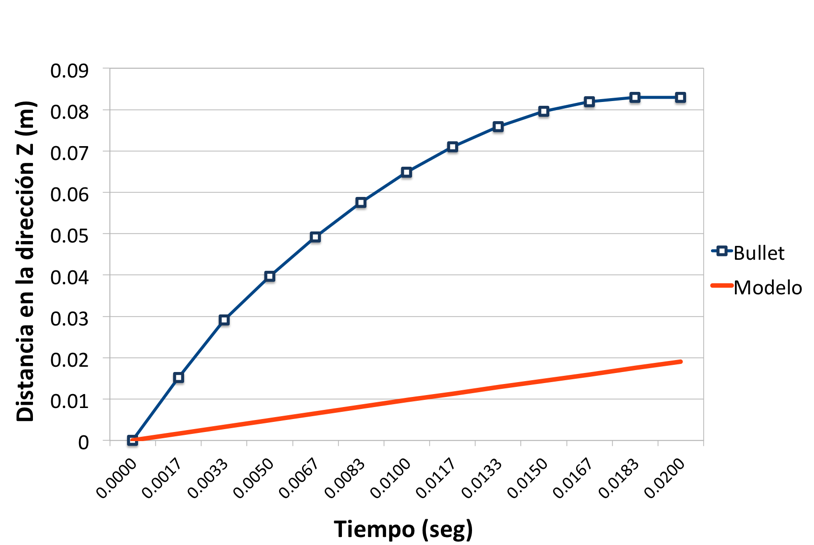
\includegraphics[width=0.6\linewidth]{image006.png} 
	\label{fig3:b} 
  }
 \vspace*{0ex}
  \subfloat[][]{
  	\centering
	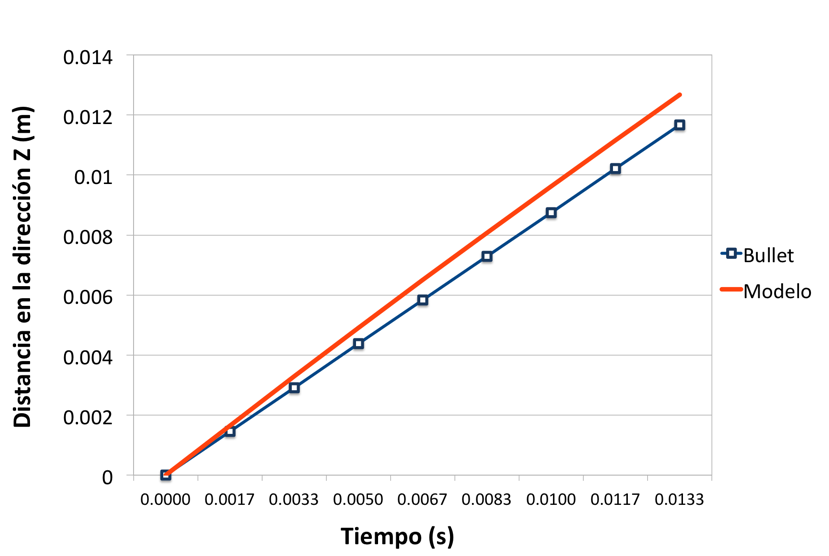
\includegraphics[width=0.6\linewidth]{image005.png} 
	\label{fig3:c} 
  }
   \captionsetup{justification=centering}
  \caption{Resultados logrados de simular el sistema descripto en Fig. \ref{fig:translatingCube}, usando $v_i = 1 \frac{m}{s}$ y: \\ (\protect\subref*{fig3:a}) $\mu_d=$0.25, (\protect\subref*{fig3:b}) $\mu_d=$0.50, y (\protect\subref*{fig3:c}) $\mu_d=$0.75}%
  \label{fig3} %
  \vspace*{0ex}
\end{figure}
\vspace{3ex}
\noindent Las Fig. \ref{fig1} y \ref{fig2} demuestran que los resultados de las pruebas fueron favorables. Los valores obtenidos a partir de la simulaci\'on se corresponden (en mayor o menor medida) con los alcanzados a partir del modelo matem\'atico. Esto es un indicador de que \textit{Bullet} debe estar usando dichos modelos para ejecutar las simulaciones. Vale observar que, cuanto mayor es la velocidad inicial ($v_{i}$), mayor es la similitud entre los dos casos.\\
No obstante, los gr\'aficos que corresponden a la Fig. \ref{fig3}, presentan una discrepancia mayor entre la simulaci\'on y el modelo. Este hecho puede deberse al mecanismo utilizado por \textit{Bullet} para resolver la fricci\'on de un cuerpo a velocidades muy bajas.

\paragraph{Verificaci\'on del coeficiente de restituci\'on}\mbox{}

El segundo ensayo simula una esfera a una altura determinada sobre el suelo, que tiene una velocidad inicial ($v_{i}$) en el eje perpendicular al piso, y que eventualmente colisiona contra el mismo.
Se desea comprobar que, la colisi\'on entre el cuerpo y el suelo respete que la velocidad final ($v_{f}$) de la esfera despu\'es del choque, sea proporcional a su coeficiente de restituci\'on ($e$) dado por la ecuaci\'on:
 \begin{equation}
 \label{eq:restitution_coef}
  e = \frac{v_f}{v_i} 
\end{equation}
\\
Para efectuar la colisi\'on con el suelo, se emple\'o una esfera s\'olida ubicada a 4 metros del suelo, cuya masa y radio son $m_{sphere} = 1\ kg$ y $r_{sphere}=1\ m$,
respectivamente (Fig. \ref{fig:fallingBall}).  A la esfera se le asigna, adem\'as, un coeficiente de restituci\'on determinado.\\
Se eligi\'o un ambiente sin gravedad ($g = 0 \frac{m}{s^2}$). De esta forma, se podr\'a tener en cuenta s\'olo la velocidad inicial ($v_{i}$) y la velocidad final ($v_{f}$) para el c\'alculo del coeficiente de restituci\'on ($e$) (ver ec. \eqref{eq:restitution_coef}).\\
El intervalo de tiempo f\'isico (o \textit{timestep}) utilizado es $\Delta t=$0.001 $s$. El \textit{timestep} de animaci\'on (es decir,
cada cu\'anto tiempo se guardan en un archivo los datos logrados) es $\Delta t' = $0.1 y el tiempo de simulaci\'on es de $s=100\Delta t$. El coeficiente de fricci\'on es $\mu = $0.75. \\
\begin{figure}[H]%
  \centering
  \frame{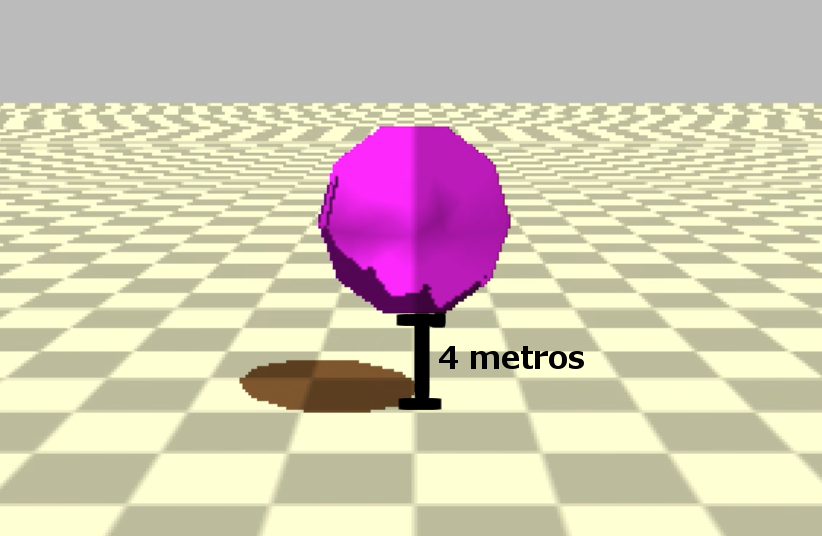
\includegraphics[width=0.4\linewidth]{fallingBall.png}}
    \caption{Visualizaci\'on del sistema de la esfera}
    \label{fig:fallingBall} 
\end{figure} 
\vspace{10pt} 
\noindent El ensayo tiene como par\'ametros de entrada: $v_{i}$ (velocidad inicial) y $e_{sim}$ (coeficiente de restituci\'on esperado). Por otro lado, se obtiene $v_{f}$ (velocidad de la esfera al finalizar la simulaci\'on); y luego se calculan $e_{medida}$ (coeficiente de restituci\'on obtenido a partir de la ec. \eqref{eq:restitution_coef}) y $\epsilon_{rel}$, que es el error relativo entre los coeficientes $e_{sim}$ y $e_{medida}$, calculado de la siguiente manera: \\
 \begin{equation}
  \epsilon_{rel} = \frac{e_{sim}-e_{medida}}{e_{sim}}
\end{equation}
\\
En la Tabla \ref{table1} se puede observar lo arrojado por los experimentos num\'ericos que se efectuaron; usando: $v_{i}= \{$ -0.5, -3.5, -4, -5 y -10$\} \frac{m}{s}$ y $e_{sim}= \{ $0.2, 0.5 y 0.8$\} $.
\begin{table}[H]%
  \centering
  	\begin{tabular}{ | c | c || c | c | c | }
	  		\hline
	  		$\boldsymbol{v_{i}}$ & $\boldsymbol{e_{sim}}$ & $\boldsymbol{v_{f}}$ & $\boldsymbol{e_{medida}}$ & $\boldsymbol{\epsilon_{rel}}$ \\
			\hline 
			\multirow{3}{*}{-0.5 $\frac{m}{s}$} & 0.2 & 0.000249 $\frac{m}{s}$& 0.000498 & 0.997\\ \cline{2-5}
								& 0.5 & 0.000219 $\frac{m}{s}$ & 0.000438 & 0.999\\ \cline{2-5}
	  							& 0.8 & 0.001037 $\frac{m}{s}$ & 0.002074 & 0.997 \\ \cline{2-5}
	  		\hline 
			\hline
			\multirow{3}{*}{-3.5 $\frac{m}{s}$} & 0.2 & 0.000057 $\frac{m}{s}$ & 0 & 1\\ \cline{2-5}
	  							& 0.5 & 0.000018 $\frac{m}{s}$ & 0 & 1 \\ \cline{2-5}
								& 0.8 & 0.3 $\frac{m}{s}$ & 0.0857 & 0.893 \\ \cline{2-5}
	  		\hline
			\hline
			\multirow{3}{*}{-4 $\frac{m}{s}$} & 0.2 & 0.000473 $\frac{m}{s}$ & 0.00012 & 1\\ \cline{2-5}
	  							& 0.5 & 0.000424 $\frac{m}{s}$ & 0.00011 & 1 \\ \cline{2-5}
	  							& 0.8 & 1.23 $\frac{m}{s}$ & 0.3 & 0.625 \\ \cline{2-5}
	  		\hline
			\hline
			\multirow{3}{*}{-5 $\frac{m}{s}$} & 0.2 & 1 $\frac{m}{s}$ & 0.2 & 0 \\ \cline{2-5}
	  							& 0.5 & 2.5 $\frac{m}{s}$ & 0.5 & 0 \\ \cline{2-5}
	  							& 0.8 & 4 $\frac{m}{s}$ & 0.8 & 0 \\ \cline{2-5}
			\hline
			\hline
			\multirow{3}{*}{-10 $\frac{m}{s}$} & 0.2 & 2 $\frac{m}{s}$ & 0.2 & 0\\ \cline{2-5}
	  							& 0.5 & 5 $\frac{m}{s}$ & 0.5 & 0 \\ \cline{2-5}
	  							& 0.8 & 8 $\frac{m}{s}$ & 0.8 & 0 \\ \cline{2-5}
			\hline
	\end{tabular}
  \captionsetup{justification=centering}
  \caption{Coeficientes de restituci\'on obtenidos ($e_{medida}$) de simular el sistema descripto en Fig. \ref{fig:fallingBall}}%
  \label{table1}%
\end{table}
\noindent Los resultados exponen una limitaci\'on del motor f\'isico: no representa correctamente las colisiones el\'asticas entre esferas y cuerpos r\'igidos, que ocurren a velocidades bajas. Esto queda en evidencia en la Tabla \ref{table1}. En cada una de ellas el error fue de casi 1. La raz\'on por la que ocurre este hecho se debe a que \textit{Bullet} utiliza un algoritmo de colisi\'on que frena la velocidad de un objeto que est\'a a punto de colisionar. Haciendo esto puede evitar que los s\'olidos se traspasen y de esta forma se pueden realizar c\'alculos de fuerza m\'as precisos. \\
En el caso de los ensayos, las esferas poseen una velocidad muy baja, cuando est\'an a punto de colisionar \textit{Bullet} reduce a\'un m\'as esta velocidad y eventualmente quedan con una velocidad tan baja que al chocar contra el suelo se aplica el efecto restitutivo a esta velocidad casi nula y se resuelve que la esfera debe quedar en reposo, cuando en realidad deber\'ia poseer una velocidad baja, pero no despreciable.


\subsubsection{Ventajas}
Las ventajas del motor f\'isico son:
\begin{itemize}[leftmargin=5.5mm]
\item C\'odigo abierto: mayor conocimiento sobre las f\'ormulas y m\'etodos implementados en el motor.
\item Soporte de la comunidad cient\'ifica.
\item Licencia libre.
\end{itemize}


\subsubsection{Desventajas}
Como toda herramienta, \textit{Bullet} tiene aspectos negativos, entre los que se encuentran: 
\begin{itemize}[leftmargin=5.5mm]
\item Documentaci\'on poco clara y desordenada.
\item Debido a que la f\'isica se aproxima usando m\'etodos num\'ericos que contienen error, las simulaciones son no determin\'isticas.
\item Utilizar una librer\'ia gr\'afica como \textit{OpenGL} acoplada a una simulaci\'on  de \textit{Bullet}, puede producir resultados distintos, que si se usa un programa de visualizaci\'on externo como OVITO.
\end{itemize}


\subsection{Librer\'ia de algoritmos gen\'eticos}

%\begin{adjustwidth}{1.2cm}{0cm}
Se utiliz\'o la conocida librer\'ia de algoritmos gen\'eticos para C++ GaLib, desarrollada por Matthew Wall del MIT \cite{LinkGaLib}. \\
Ofrece funcionalidades como: programaci\'on paralela, diversos m\'etodos de selecci\'on (\textit{elite}, \textit{roulette}), estrategias de reemplazo (de padres, aleatorio, del peor), entre otras.\\
Cabe aclarar que, antes de optar por GaLib, se hab\'ia adoptado la librer\'ia Kataklinger, pero finalmente fue descartada, debido a errores o \textit{bugs} en la misma (y que, cada vez, resultaban ser m\'as inmanejables).

%\end{adjustwidth}

\subsection{C\'odigo fuente}

%\begin{adjustwidth}{1.2cm}{0cm}
Al estar \textit{Bullet} implementado en C++, el c\'odigo fuente tambi\'en est\'a desarrollado en ese lenguaje. En \textit{Bullet}, se define un \textit{World} (o mundo f\'isico) en donde se puede insertar, entre otras cosas, cuerpos r\'igidos. En este caso en particular, el mundo consta de un plano  (el suelo), y  el b\'ipedo (compuesto por cuerpos r\'igidos y otros elementos f\'isicos) ubicado sobre \'el. \\
El \textit{software} creado incluye: construcci\'on del humanoide, siendo \'este capaz de desplazarse por medio de actuadores (que se ver\'an en la Secci\'on \ref{actuadores}); el desarrollo del algoritmo gen\'etico (definici\'on de los individuos, funci\'on de \textit{fitness}, m\'etodos de selecci\'on, etc.); visualizaci\'on gr\'afica del mejor humanoide logrado por el algoritmo gen\'etico; y la posibilidad de realizar gr\'aficos referidos a la evoluci\'on del algoritmo gen\'etico (\textit{fitness} por cada generaci\'on, etc.). \\
Se acompa\~nan a esta presentaci\'on: el c\'odigo fuente y el manual de instalaci\'on y uso.

%\end{adjustwidth}

%\end{adjustwidth}


%----------------------------------------------------------------------------------------
%	SECTION 3 - MODELO UTILIZADO
%----------------------------------------------------------------------------------------

\section{Modelo utilizado}

%\begin{adjustwidth}{1.1cm}{0cm}
Dentro de los diversos modelos existentes (\cite{Wojtyra}\cite{flexibleMuscle}), en este trabajo se procur\'o utilizar uno que fuera sencillo pero representativo a la vez.\\ 
Se modela al cuerpo del b\'ipedo, con el motor \textit{Bullet Physics}, como un conjunto de segmentos unidos entre s\'i por articulaciones. A cada uno de ellos se les aplica un torque en el centro de masa de cada segmento (denominado actuador). Que la caminata se produzca o no, depende del tipo de actuador empleado (la funci\'on utilizada para el torque), y de sus par\'ametros. El objetivo es encontrar dichos par\'ametros. Para eso se usan los algoritmos gen\'eticos, un m\'etodo de inteligencia artificial. De este modo se obtiene, de forma an\'aloga a la selecci\'on natural, los individuos que mejor se adapten a la caminata. Tanto los actuadores como el algoritmo gen\'etico se explicar\'an m\'as adelante.

\subsection{Composici\'on f\'isica del humanoide}
Como ya se expres\'o, el humanoide fue modelado en \textit{Bullet} como un conjunto de segmentos (cuerpos r\'igidos), unidos entre s\'i por articulaciones. \\
Sobre la base de la anatom\'ia humana, se dividi\'o el cuerpo del humano virtual en: cabeza, tronco, miembro superior (brazo, antebrazo y mano), pelvis y miembro inferior (muslo, pierna y pie). \\
A los fines de este proyecto, s\'olo se consideraron pelvis y miembro inferior (Fig. \ref{fig:humanoid_segments}).
\begin{figure}[H]%
  \centering
  \frame{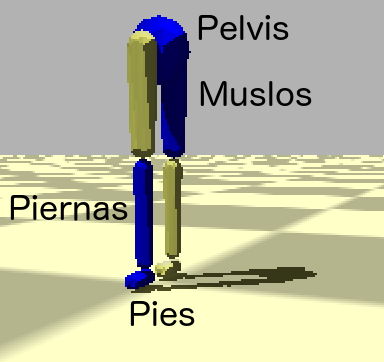
\includegraphics[width=0.28\linewidth]{humanoid_segments.png}}  
    \caption{Segmentos del humanoide}
    \label{fig:humanoid_segments}
\end{figure} 
\noindent En la Tabla \ref{table2} se presenta la composici\'on f\'isica de cada uno de los segmentos del humano virtual, de acuerdo a la biomec\'anica \cite{biomechanics}.
\begin {table}[H]
	\begin{center}
	\resizebox{\linewidth}{!}{%
		\begin{tabular}{ | c | c | c || c | c | c | c | c |}
	  		 \cline{4-8}
	  		\multicolumn{3}{ c |}{} & \textbf{Cantidad} & \textbf{Forma} & \textbf{Largo (en m)} & \textbf{Masa (en kg)} & \textbf{Uniones}\\
	  		\hline 
	  		\multirow{4}{*}{\textbf{\rotatebox[origin=c]{90}{Segmento}  } } & \multicolumn{2}{| c ||}{ \textbf{Pelvis} } & 1 & Esf\'erica & 0.08655 & 9.9718 & Cadera\\
												\cline{2-8}
	  										      &\multirow{3}{*}{\parbox{1.45cm}{ \textbf{Miembro inferior} }  } & \textbf{Muslo} & 2 & Esfero-cil\'indrica & 0.4015 & 10.3368 & Cadera y Rodilla\\
	  											 \cline{3-8}
	  										          &  & \textbf{Pierna} & 2 & Esfero-cil\'indrica &  0.4015 & 3.1609 & Rodilla y Tobillo\\
	  											  \cline{3-8}
	  											 &	& \textbf{Pie} & 2 & Esfero-cil\'indrica & - & 1.0001 & Tobillo\\
	  		\hline
			
		\end{tabular}
		}
		\caption{Composici\'on f\'isica de cada segmento del humanoide}
		\label{table2}
	\end{center}
\end{table}

%\end{adjustwidth}

\subsection{Articulaciones}
Para unir los distintos segmentos entre s\'i, se utilizaron articulaciones bisagra con 1 grado de libertad, en el eje X, para que los segmentos puedan moverse en dos ejes: el Z, donde ocurre la caminata, y el Y, perpendicular al piso (Fig. \ref{fig:seg_and_art}(\protect\subref*{fig7:a}) y (\protect\subref*{fig7:b})). \\
A su vez, para cada caso en particular, se definieron cotas para los \'angulos que pueden existir entre los segmentos (ver Tabla \ref{table_articulaciones}). Esto es muy importante, no s\'olo porque se adec\'ua a datos biol\'ogicos, sino porque, de otro modo la caminata no podr\'ia lograrse: si los \'angulos son demasiado altos, la caminata se produce girando las piernas por encima de la pelvis; si por el contrario, son demasiado bajos, las piernas van a estar muy r\'igidas, originando pocos pasos y muy cortos.\\
Asimismo, se le impide rotar a la pelvis, y se restringe la amplitud con la que puede moverse la cadera (de $\frac{-\pi}{4}$ a $\frac{\pi}{4}$). Esto se realiza porque, en caso contrario, el b\'ipedo necesitar\'ia un sistema de control para mantener el equilibrio, y eso excede el alcance de este trabajo.

\begin{figure}[H]%
  \centering
  \subfloat[][]{
  	\centering
	  \frame{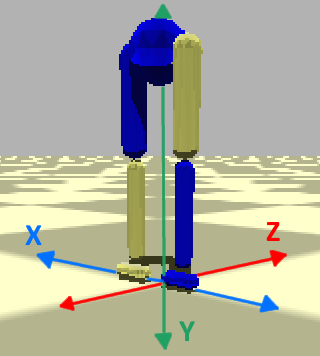
\includegraphics[width=0.28\linewidth]{humanoid_axis.png}} 
	\label{fig7:a} 
  }
  \qquad
  \subfloat[][]{
  	\centering
	  \frame{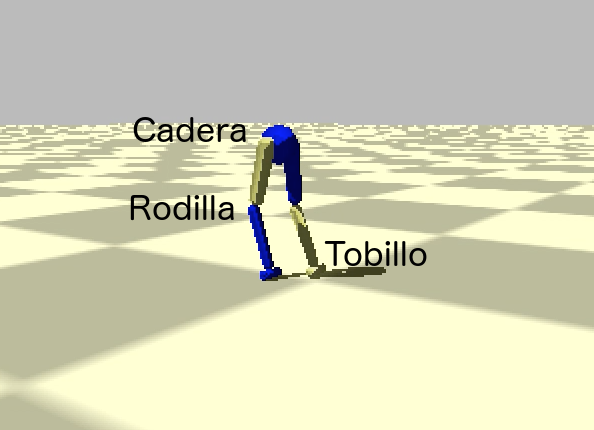
\includegraphics[width=0.38\linewidth]{humanoid_articulations.png}}
	\label{fig7:b} 
  }
  \caption{Humanoide dise\~nado: (\protect\subref*{fig7:a}) ejes, y (\protect\subref*{fig7:b}) articulaciones}%
  \label{fig:seg_and_art} %
\end{figure}

%\begin {table}[H]
%	\begin{center}
%		\begin{tabular}{ | c || c | c | c | c | c |}
%	  		 \hline
%	  		 \textbf{Articulaci\'on} & \textbf{\'Angulo m\'inimo} & \textbf{\'Angulo m\'aximo}\\
%	  		\hline
%			Cadera & -$\frac{\pi}{4}$ & $\frac{\pi}{4}$\\
%			\hline
%			Rodilla & -$\pi$ & $\pi$ \\
%			\hline
%	  		Tobillo & 0 & 0 \\
%	  		\hline		
%		\end{tabular}
%		\caption{Rango de valores de \'angulo de cada articulaci\'on del humanoide}
%		\label{table_articulaciones}
%	\end{center}
%\end{table}

\begin {table}[H]
	\begin{center}
		\begin{tabular}{ | c | c || c | c |}
	  		 \cline{3-4}
	  		 \multicolumn{2}{ c |}{}  & \textbf{\'Angulo m\'inimo} & \textbf{\'Angulo m\'aximo}\\
	  		\hline
			\multirow{3}{*}{\textbf{Articulaci\'on}} & \textbf{Cadera} & -$\frac{\pi}{4}$ & $\frac{\pi}{4}$\\
			\cline{2-4}
			& \textbf{Rodilla} & -$\pi$ & $\pi$ \\
			\cline{2-4}
	  		& \textbf{Tobillo} & 0 & 0 \\
	  		\hline		
		\end{tabular}
		\caption{Rango de valores de \'angulo de cada articulaci\'on del humanoide}
		\label{table_articulaciones}
	\end{center}
\end{table}

%----------------------------------------------------------------------------------------
%	SECTION 4 - ACTUADORES
%----------------------------------------------------------------------------------------

\section{Actuadores}
\label{actuadores}

A cada uno de los segmentos correspondientes al muslo y la pierna del b\'ipedo, se le aplica un torque (o actuador) en el eje X (perpendicular a la trayectoria), como se ve en Fig \ref{fig:actuator}. As\'i, pueden moverse para arriba o para abajo (con respecto a la articulaci\'on a la que pertenecen). \\
A fin de simplificar el modelo, el humanoide tiene el mismo tipo de actuador utilizado en todos los segmentos.\\
Es necesario aclarar que la caminata producida por el humanoide es plana (en 2D). Esto se debe a que la trayectoria pensada para el b\'ipedo es una l\'inea recta, y logrando que los segmentos se muevan en un solo eje es suficiente para cumplir con dicha trayectoria. Tambi\'en contribuye el hecho de que el torque se aplique en una sola dimensi\'on. Por otra parte, los actuadores definidos a continuaci\'on son peri\'odicos, y por eso no se pueden aplicar en el eje Z de los segmentos (se necesitar\'ian actuadores reactivos, para poder detectar cuando el humanoide se est\'a cayendo, etc.). Para indicar el m\'odulo de dicho torque, se dise\~naron diferentes funciones (todas ellas peri\'odicas), mencionadas en las subsecciones que siguen. \\
\begin{figure}[H]%
  \centering
  \frame{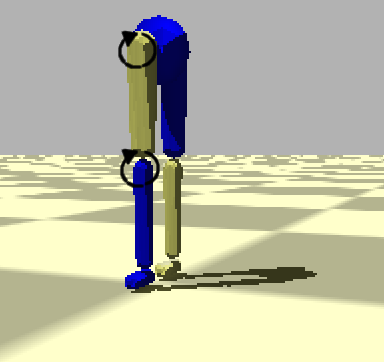
\includegraphics[width=0.3\linewidth, height=0.3\linewidth]{actuators.png}}
    \caption{Aplicaci\'on de los actuadores en los segmentos del b\'ipedo}
    \label{fig:actuator} 
\end{figure} 

\subsection{Gen\'erico}
Es el actuador m\'as sencillo, tanto matem\'atica como computacionalmente.
\begin{equation}
  f(t) =  A_1 \sin(\omega_1t+\phi)+A_2 \cos(\omega_2t+\phi)+C
\end{equation}
donde $f(t)$ es la funci\'on del actuador evaluada en el instante de tiempo $t$, $A_{1}$ y $A_{2}$ son amplitudes, $\omega_1$ y $\omega_2$ son frecuencias (en $\frac{1}{s}$), $\phi$ es la fase en radianes, y $C$ es un t\'ermino independiente (ver Fig. \ref{actuadores:generico} (\subref*{actuadores:generico_muslo}) y (\subref*{actuadores:generico_pierna})).\\
La fase $\phi$ es la misma en el seno y en el coseno, para evitar que se formen otro tipo de funciones no c\'iclicas.

\begin{figure}[H]%
  \centering
  \subfloat[][]{
  	\centering
	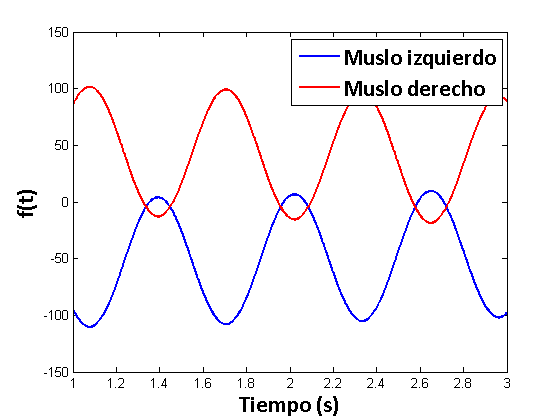
\includegraphics[width=0.5\linewidth, height=0.3\linewidth]{graficos_actuadores/actuador_generico_muslo.png} 
	\label{actuadores:generico_muslo} 
  }%
  \subfloat[][]{
  	\centering
	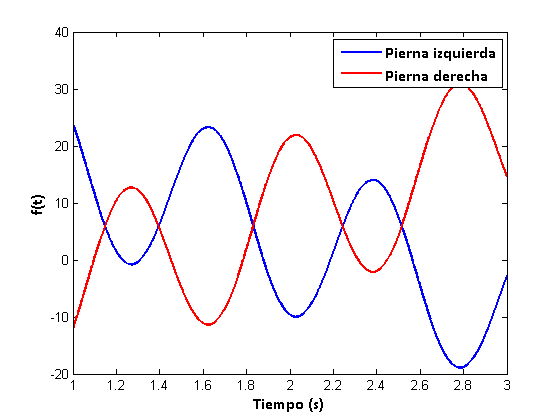
\includegraphics[width=0.5\linewidth, height=0.3\linewidth]{graficos_actuadores/actuador_generico_pierna.png} 
	\label{actuadores:generico_pierna} 
  }
  \captionsetup{justification=centering}
  \caption{Ejemplo de actuador gen\'erico aplicado en: (\protect\subref*{actuadores:generico_muslo}) muslo, y (\protect\subref*{actuadores:generico_pierna}) pierna}%
  \label{actuadores:generico} %
\end{figure}

\subsection{Coseno doble frecuencia}
Basada en \cite{Cuadrupedo}, esta funci\'on peri\'odica utiliza medio ciclo de una funci\'on sinusoidal, y medio ciclo de otra (ambas pueden tener frecuencias distintas). Esto podr\'ia tener sentido porque en una caminata, un miembro inferior primero avanza hacia adelante y luego se extiende hacia atr\'as, y es razonable que esos dos movimientos se produzcan a frecuencias distintas  (Fig. \ref{actuadores:coseno_doble_frecuencia} (\subref*{actuadores:coseno_doble_frecuencia_muslo}) y (\subref*{actuadores:coseno_doble_frecuencia_pierna})).\\
La idea es lograr una funci\'on peri\'odica a partir de una que no lo es (ya que $t$ es lineal). Para eso, se utiliza la funci\'on $\psi (t)$ (ec. \eqref{eq:phi}) que aplica una transformaci\'on a los n\'umeros reales, para que se encuentren dentro del rango del ciclo completo (con las dos frecuencias). $\omega$ es la frecuencia de $f(t)$ (ec. \eqref{eq:ft}), que utiliza medio ciclo con frecuencia $\omega_1$ y medio ciclo con frecuencia $\omega_2$.
\begin{equation} 
\label{eq:phi}
\begin{aligned}[c]
\psi (t) = t+ \phi- \floor[\Bigg]{ \frac{t+\phi}{\pi/\omega_1+\pi/\omega_2} } (\pi/\omega_1+\pi/\omega_2) 
 \end{aligned}
 \qquad
 \begin{aligned}[c]
 \psi: \mathbb{Re} \rightarrow \bigg[0, \frac{2\pi}{\omega}\bigg] 
 \end{aligned}
\end{equation}
 \\
\begin{equation}
\omega = \frac{2\omega_1 \omega_2}{\omega_1+\omega_2} 
 \end{equation}
\\
\begin{equation}
\label{eq:ft}
f(t) =  \left\{
\begin{array}{ll}
      A \cos(\omega_1 \psi(t))+C & \mbox{si $\omega_1 \psi(t) < \pi$}  \\
      A \cos(\omega_2 (\psi(t) - (\pi/\omega_1) + (\pi/\omega_2 ) ) )+C & \mbox{en otro caso$$} \\
\end{array} 
\right. 
 \end{equation}

\begin{figure}[H]%
  \centering
  \subfloat[][]{
  	\centering
	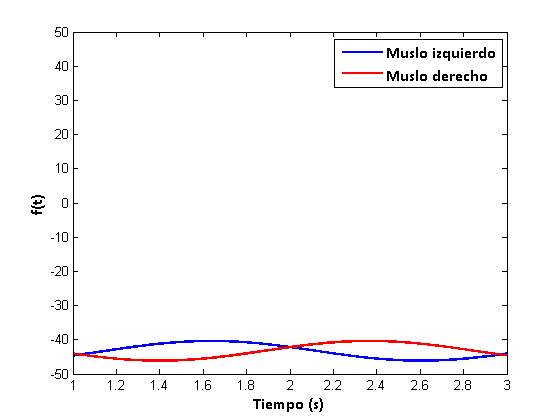
\includegraphics[width=0.5\linewidth, height=0.3\linewidth]{graficos_actuadores/actuador_coseno_doble_frecuencia_muslo.png} 
	\label{actuadores:coseno_doble_frecuencia_muslo} 
  }%
  \subfloat[][]{
  	\centering
	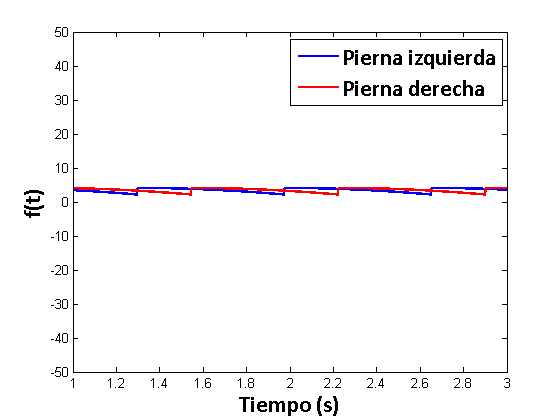
\includegraphics[width=0.5\linewidth, height=0.3\linewidth]{graficos_actuadores/actuador_coseno_doble_frecuencia_pierna.png} 
	\label{actuadores:coseno_doble_frecuencia_pierna} 
  }
  \captionsetup{justification=centering}
  \caption{Ejemplo de actuador coseno doble frecuencia aplicado en: (\protect\subref*{actuadores:coseno_doble_frecuencia_muslo}) muslo, y (\protect\subref*{actuadores:coseno_doble_frecuencia_pierna}) pierna}%
  \label{actuadores:coseno_doble_frecuencia} %
\end{figure}


\subsection{Fourier de orden 2}
Este actuador utiliza una serie de Fourier de dos t\'erminos. 
\begin{equation}
  f(t) =  A_1 \sin(\omega t+\phi)+B_1 \cos(\omega t+\phi)+A_2 \sin(2\omega t+\phi)+B_2 \cos(2\omega t+\phi)+C
\end{equation}
donde $A_{1}$, $A_{2}$, $B_{1}$ y $B_{2}$ son amplitudes y $\omega$ es frecuencia (en $\frac{1}{s}$) (ver Fig. \ref{actuadores:fourier2} (\subref*{actuadores:fourier2_muslo}) y (\subref*{actuadores:fourier2_pierna})).
\begin{figure}[H]%
  \centering
  \subfloat[][]{
  	\centering
	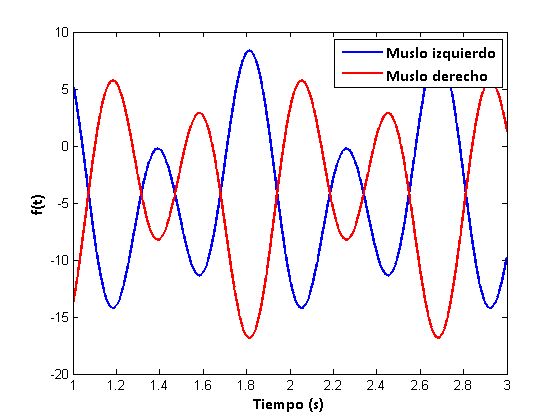
\includegraphics[width=0.5\linewidth, height=0.3\linewidth]{graficos_actuadores/actuador_fourier_2_muslo.png} 
	\label{actuadores:fourier2_muslo} 
  }%
  \subfloat[][]{
  	\centering
	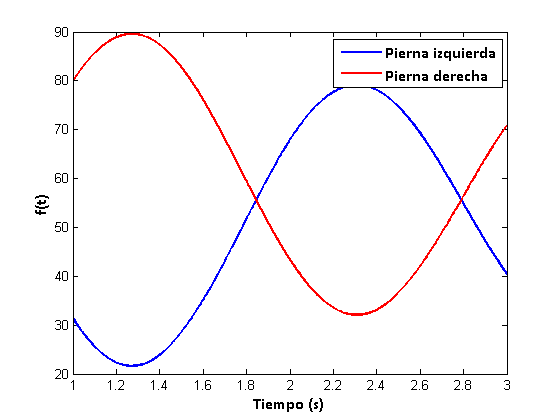
\includegraphics[width=0.5\linewidth, height=0.3\linewidth]{graficos_actuadores/actuador_fourier_2_pierna.png} 
	\label{actuadores:fourier2_pierna} 
  }
  \captionsetup{justification=centering}
  \caption{Ejemplo de actuador fourier de orden 2 aplicado en: (\protect\subref*{actuadores:fourier2_muslo}) muslo, y (\protect\subref*{actuadores:fourier2_pierna}) pierna}%
  \label{actuadores:fourier2} %
\end{figure}

\subsection{Fourier de orden 9}
Es una extensi\'on del actuador anterior, pero con 9 t\'erminos. Por ser de mayor grado, brinda una mayor precisi\'on. Sin embargo, es m\'as dificil de manejar computacionalmente; y, adem\'as, que sea m\'as preciso no garantiza que con \'el se pueda lograr una buena caminata  (ver Fig. \ref{actuadores:fourier9} (\subref*{actuadores:fourier9_muslo}) y (\subref*{actuadores:fourier9_pierna})).\\
\begin{equation}
\begin{split}
  f(t) = &   A_1 \sin(\omega t+\phi)+B_1 \cos(\omega t+\phi)+A_2 \sin(2\omega t+\phi)+B_2 \cos(2\omega t+\phi) \\
  &+A_3 \sin(3\omega t+\phi)+B_3 \cos(3\omega t+\phi)+A_4 \sin(4\omega t+\phi)+B_4 \cos(4\omega t+\phi) \\ 
  &+A_5 \sin(5\omega t+\phi)+B_5 \cos(5\omega t+\phi)+A_6 \sin(6\omega t+\phi)+B_6 \cos(6\omega t+\phi) \\
  &+A_7 \sin(7\omega t+\phi)+B_7 \cos(7\omega t+\phi)+A_8 \sin(8\omega t+\phi)+B_8 \cos(8\omega t+\phi) \\
  &+A_9 \sin(9\omega t+\phi)+B_9 \cos(9\omega t+\phi) + C
\end{split}
\end{equation}
donde $A_{i}$ y $B_{i}$ con $1 \leq i \leq 9$ son amplitudes.
\begin{figure}[H]%
  \centering
  \subfloat[][]{
  	\centering
	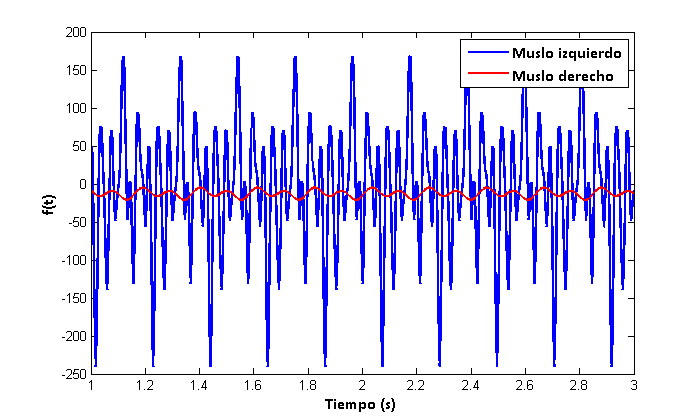
\includegraphics[width=0.44\linewidth,  height=0.3\linewidth]{graficos_actuadores/actuador_fourier_9_muslo.png} 
	\label{actuadores:fourier9_muslo} 
  }%
  \subfloat[][]{
  	\centering
	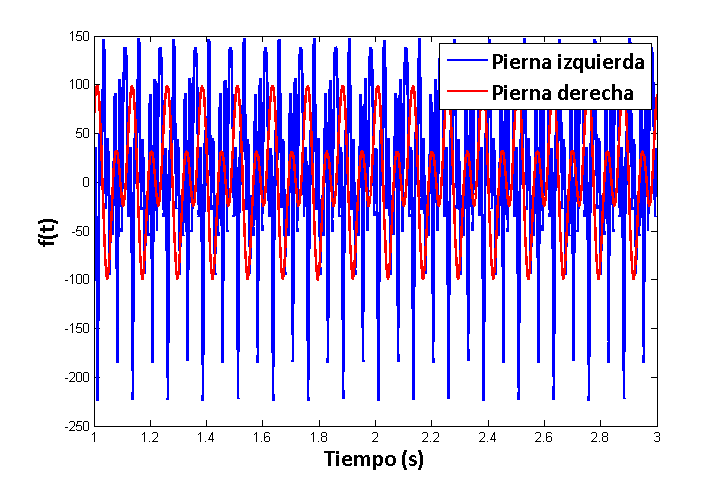
\includegraphics[width=0.56\linewidth, height=0.3\linewidth]{graficos_actuadores/actuador_fourier_9_pierna.png} 
	\label{actuadores:fourier9_pierna} 
  }
  \captionsetup{justification=centering}
  \caption{Ejemplo de actuador fourier de orden 9 aplicado en: (\protect\subref*{actuadores:fourier9_muslo}) muslo, y (\protect\subref*{actuadores:fourier9_pierna}) pierna}%
  \label{actuadores:fourier9} %
\end{figure}


%----------------------------------------------------------------------------------------
%	SECTION 5 - CONDICIONES INICIALES Y DE CONTORNO
%----------------------------------------------------------------------------------------

\section{Condiciones iniciales y de contorno}
Como las funciones peri\'odicas se\~naladas en los actuadores, no fueron suficientes para lograr la caminata, se le adosaron las funciones que se detallan seguidamente. 
\subsection{Funci\'on partida}
El andar del humanoide es c\'iclico. Sin embargo, por la posici\'on inicial del individuo, se requiere para el tiempo del primer paso, una funci\'on distinta a la del resto de la caminata. El tipo de funci\'on puede ser cualquiera de los actuadores vistos anteriormente (pero no necesariamente con los mismos valores de amplitud, frecuencia y fase asignados a las piernas). Empero, se utiliz\'o la funci\'on vista en el actuador gen\'erico. \\
Por otra parte, para simplificar el modelo, se decidi\'o  que el tiempo considerado para el primer paso sea fijo, y de 0.7 segundos. Dicho valor fue extra\'ido de forma experimental.

\subsection{Fase sincronizada}
En una caminata, las piernas deben guardar simetr\'ia: mientras una va hacia adelante, la otra va hacia atr\'as (y viceversa). Esto, de acuerdo con  los actuadores definidos en la secci\'on anterior, implica que las funciones de movimiento de cada pierna est\'en desfasadas en medio ciclo ($\frac{\pi}{2}$):\\
\begin{equation}
f_{i}(t) =  f(t)
 \end{equation}
 \begin{equation}
f_{d}(t) =  f(t+\frac{\pi}{2})
 \end{equation}
 \\
siendo $f(t)$ la funci\'on de movimiento (o actuador) en el momento $t$, y $f_{i}$ y $f_{d}$ las funciones de la pierna izquierda y derecha, respectivamente.


%----------------------------------------------------------------------------------------
%	SECTION 6 - ALGORITMO GENETICO
%----------------------------------------------------------------------------------------

\section{Algoritmo gen\'etico}

Los algoritmos gen\'eticos son m\'etodos adaptativos, que pueden ser utilizados para resolver problemas de b\'usqueda y optimizaci\'on. Est\'an inspirados en la teor\'ia darwiniana de la selecci\'on natural. La entidad a optimizar constituye un individuo dentro de una poblaci\'on; que puede ser cruzado con otros individuos para obtener un ``hijo", que presenta caracter\'isticas de sus ``padres". A trav\'es de una funci\'on de \textit{fitness} se decide cu\'ales de ellos son los m\'as ``aptos", que luego pasar\'an a una nueva generaci\'on de individuos. Este proceso se repite hasta obtener un individuo lo suficientemente apto, que representa a la entidad optimizada.\\
El objetivo de este proyecto es optimizar la caminata del humanoide. Ergo, en el algoritmo gen\'etico aplicado, el individuo est\'a definido por rasgos del b\'ipedo, y la funci\'on de \textit{fitness} se focaliza en mejorar diversos aspectos de dicha caminata.

\subsection{Individuo}

%La informaci\'on gen\'etica de cada individuo, est\'a compuesta por dos partes: funci\'on partida (optativa) y los par\'ametros asociados a los actuadores (obligatorios). 
La informaci\'on gen\'etica de cada individuo, est\'a definida a partir de un vector que contiene de forma contigua, los par\'ametros de la funci\'on partida (optativa) y los asociados a los actuadores (obligatorios), que act\'uan sobre cada uno de los segmentos (muslos y piernas) del humano virtual.  

\subsubsection{Par\'ametros}
\label{sub:parametros}
Tanto la funci\'on partida como los actuadores tienen como par\'ametros: amplitud ($A$ o $B$); frecuencia ($\omega$); fase ($\phi$), que indica d\'onde comienza el paso y se mide en radianes;  y t\'ermino independiente ($C$). \\
La Fig. \ref{fig:individuoGraphic} muestra la estructura del individuo y su composici\'on para un humanoide con funci\'on partida y actuador gen\'erico.\\

\begin{figure}[H]%
   \centering
  \begin{tikzpicture}[scale=0.85, every node/.style={scale=0.85}]
	\def\rectanglepath[#1][#2]{-- ++(#1,0cm) -- ++(0cm,#2) -- ++(-#1,0cm) -- cycle}

	\draw (6.7,-3.05) node[font=\bf, ultra thick]{Individuo};
	\draw[thick,->] (6.7,-2) -- ++(0cm,-0.7cm) ;
	\draw[ultra thick] (5.45,-3.4) \rectanglepath[2.5cm][0.7cm];
	\draw[thick] (2.5,-2) -- ++(8.95cm,0cm) ;


	\draw (2.5,-1.15) node{Funci\'on partida};
	\draw[ultra thick] (1,-1.5) \rectanglepath[3cm][0.7cm];
	\draw[thick] (2.5,-1.5) -- ++(0cm,-0.5cm) ;
	\draw[thick,<-] (2.5,-0.8) -- ++(0cm,0.75cm) ;
	\draw[thick] (-1.55,-0.05) -- ++(8.25cm,0cm) ;


	\draw (11.45,-1.15) node{Actuador gen\'erico};
	\draw[ultra thick]  (9.85,-1.5) \rectanglepath[3.2cm][0.7cm];
	\draw[thick] (11.45,-1.5) -- ++(0cm,-0.5cm) ;
	\draw[thick,<-] (11.45,-0.8) -- ++(0cm,0.75cm) ;
	\draw[thick] (10.1,-0.05) -- ++(2.7cm,0cm) ;


	\draw (-3,0.5) \rectanglepath[2.75cm][1cm];
	\draw (-1.6,1) node{Pierna izquierda};
	\draw[thick] (-1.55,0.5) -- ++(0cm,-0.55cm) ;

	\draw (-3,2) \rectanglepath[2.75cm][1cm];
	\draw (-2.7,2.5) node{$A_1$};
	\draw (-2.3,2.5) node{$A_2$};
	\draw (-1.8,2.5) node{$\omega_{1}$};
	\draw (-1.3,2.5) node{$\omega_{2}$};
	\draw (-0.9,2.5) node{$\phi$};
	\draw (-0.5,2.5) node{$C$};
	\draw[thick,->] (-1.55,2) -- ++(0cm,-0.5cm) ;


	\draw (-0.25,0.5) \rectanglepath[2.75cm][1cm];
	\draw (1.1,1.0) node{Muslo izquierdo};
	\draw[thick] (1.2,0.5) -- ++(0cm,-0.55cm) ;


	\draw (-0.25,2) \rectanglepath[2.75cm][1cm];
	\draw (0.05,2.5) node{$A_1$};
	\draw (0.45,2.5) node{$A_2$};
	\draw (0.95,2.5) node{$\omega_{1}$};
	\draw (1.45,2.5) node{$\omega_{2}$};
	\draw (1.85,2.5) node{$\phi$};
	\draw (2.25,2.5) node{$C$};
	\draw[thick,->] (1.2,2) -- ++(0cm,-0.5cm) ;


	\draw (2.5,0.5) \rectanglepath[2.75cm][1cm];
	\draw (3.85,1.03) node{Pierna derecha};
	\draw[thick] (3.95,0.5) -- ++(0cm,-0.55cm) ;

	\draw (2.5,2) \rectanglepath[2.75cm][1cm];
	\draw (2.8,2.5) node{$A_1$};
	\draw (3.2,2.5) node{$A_2$};
	\draw (3.7,2.5) node{$\omega_{1}$};
	\draw (4.2,2.5) node{$\omega_{2}$};
	\draw (4.6,2.5) node{$\phi$};
	\draw (5.0,2.5) node{$C$};
	\draw[thick,->] (3.95,2) -- ++(0cm,-0.5cm) ;


	\draw (5.25,0.5) \rectanglepath[2.75cm][1cm];
	\draw (6.65,1.03) node{Muslo derecho};
	\draw[thick] (6.7,0.5) -- ++(0cm,-0.55cm) ;

	\draw (5.25,2) \rectanglepath[2.75cm][1cm];
	\draw (5.55,2.5) node{$A_1$};
	\draw (5.95,2.5) node{$A_2$};
	\draw (6.45,2.5) node{$\omega_{1}$};
	\draw (6.95,2.5) node{$\omega_{2}$};
	\draw (7.35,2.5) node{$\phi$};
	\draw (7.75,2.5) node{$C$};
	\draw[thick,->] (6.7,2) -- ++(0cm,-0.5cm) ;


	\draw (8.7,0.5) \rectanglepath[2.75cm][1cm];
	\draw (10.1,1.02) node{Pierna};
	\draw[thick] (10.1,0.5) -- ++(0cm,-0.55cm) ;

	\draw (8.7,2) \rectanglepath[2.75cm][1cm];
	\draw (9.0,2.5) node{$A_1$};
	\draw (9.4,2.5) node{$A_2$};
	\draw (9.9,2.5) node{$\omega_{1}$};
	\draw (10.4,2.5) node{$\omega_{2}$};
	\draw (10.8,2.5) node{$\phi$};
	\draw (11.2,2.5) node{$C$};
	\draw[thick,->] (10.1,2) -- ++(0cm,-0.5cm) ;


	\draw (11.45,0.5) \rectanglepath[2.75cm][1cm];
	\draw (12.85,1.02) node{Muslo};
	\draw[thick] (12.8,0.5) -- ++(0cm,-0.55cm) ;

	\draw (11.45,2) \rectanglepath[2.75cm][1cm];
	\draw (11.75,2.5) node{$A_1$};
	\draw (12.15,2.5) node{$A_2$};
	\draw (12.65,2.5) node{$\omega_{1}$};
	\draw (13.15,2.5) node{$\omega_{2}$};
	\draw (13.55,2.5) node{$\phi$};
	\draw (13.95,2.5) node{$C$};
	\draw[thick,->] (12.8,2) -- ++(0cm,-0.5cm) ;

  \end{tikzpicture}
  \vspace{5pt}
  \caption{Esquema de un individuo - Ejemplo}
  \label{fig:individuoGraphic} 
\end{figure}

\subsubsection{Valores}

Cada uno de los segmentos tiene una composici\'on f\'isica distinta (largo, masa, etc.), raz\'on por la cual no necesariamente sus genes deban tener los mismos rangos de valores, tal como puede apreciarse en las Tablas \ref{table3} y \ref{table4}. \\
\begin{table}[H]%
  \centering
  	\begin{tabular}{ | c | c || c | c | }
	  		\hline
	  		\textbf{Segmento} & \textbf{Tipo de gen} & \textbf{M\'inimo} & \textbf{M\'aximo} \\
			\hline
			Muslo & Amplitud & -30 & 30\\
			\hline
			Pierna & Amplitud & -60 & 60\\ 
			\hline
	  		Muslo y Pierna & Frecuencia & 0.01 & 10 \\ 
	  		\hline
			Muslo y Pierna & Fase & $-\pi$ & $\pi$ \\ 
			\hline
			Muslo y Pierna & T\'ermino independiente & -10 & 10 \\ 
			\hline
	\end{tabular}
  \captionsetup{justification=centering}
  \caption{Rango de valores que puede tomar cada gen, para la funci\'on partida}%
  \label{table4}%
\end{table}
\vspace{1pt}

\begin{table}[H]%
  \centering
  	\begin{tabular}{ | c | c | c || c | c | }
	  		\hline
	  		\textbf{Actuador} & \textbf{Segmento} & \textbf{Tipo de gen} & \textbf{M\'inimo} & \textbf{M\'aximo} \\
			\hline
			\multirow{5}{*}{Gen\'erico} & Muslo & Amplitud & -30 & 30\\ \cline{2-5}
								&Pierna & Amplitud & -60 & 60\\ \cline{2-5}
	  							& Muslo y Pierna & Frecuencia & 0.01 & 10 \\ \cline{2-5}
	  							&Muslo y Pierna & Fase & $-\pi$ & $\pi$ \\ \cline{2-5}
								& Muslo y Pierna & T\'ermino independiente & -10 & 10 \\ 
	  		\hline 
			\hline
			\multirow{5}{*}{Coseno doble frecuencia} & Muslo & Amplitud & -50 & 50\\ \cline{2-5}
								& Pierna & Amplitud & -30 & 30\\ \cline{2-5}
	  							& Muslo y Pierna & Frecuencia & 0.01 & 5 \\ \cline{2-5}
	  							&Muslo y Pierna & Fase & $-\pi$ & $\pi$ \\ \cline{2-5}
								& Muslo y Pierna & T\'ermino independiente & -30 & 30 \\ \cline{2-5}
			\hline 
			\hline					
			\multirow{5}{*}{Fourier de orden 2} & Muslo & Amplitud & -60 & 60\\ \cline{2-5}
	  							&Pierna & Amplitud & -30 & 30 \\ \cline{2-5}
								& Muslo y Pierna & Frecuencia & 0.01 & 10 \\ \cline{2-5}
	  							&Muslo y Pierna & Fase & $-\pi$ & $\pi$ \\ \cline{2-5}
								& Muslo y Pierna & T\'ermino independiente & -10 & 10 \\
	  		\hline
			\hline
			\multirow{4}{*}{Fourier de orden 9} & Muslo y Pierna & Amplitud & -60 & 60\\ \cline{2-5}
	  							& Muslo y Pierna & Frecuencia & 0.1 & 2 \\ \cline{2-5}
	  							&Muslo y Pierna & Fase & $-\pi$ & $\pi$ \\ \cline{2-5}
								& Muslo y Pierna & T\'ermino independiente & -10 & 10 \\
			
			\hline
	\end{tabular}
  \captionsetup{justification=centering}
  \caption{Rango de valores que puede tomar cada gen, seg\'un el tipo de actuador }%
  \label{table3}%
\end{table}



\subsubsection{Implementaci\'on de individuos}
\label{individuos_implementacion}
Para favorecer el an\'alisis de las distintas caracter\'isticas arriba indicadas, se implementaron varios individuos, cada uno de ellos con propiedades distintas (Tabla \ref{table5}). \\
%\begin{table}[H]%
%  \centering
 % 	\begin{tabular}{ | c || c | c | c | }
%	  		\hline
%	  		\textbf{Individuo} & \textbf{Actuador} & \textbf{Funci\'on Partida} & \textbf{Fase Sincronizada} \\
%			\hline 
%			\hline
%			\textbf{Tipo 1} & Gen\'erico & No & S\'i\\ 
%	  		\hline 
%			\textbf{Tipo 2} & Gen\'erico & S\'i & S\'i\\ 
%	  		\hline 
%			\textbf{Tipo 3} & Fourier de orden 2 & S\'i & S\'i\\ 
%	  		\hline 
%			\textbf{Tipo 4} & Fourier de orden 9 & S\'i & S\'i\\ 
%	  		\hline 
%			\textbf{Tipo 5} & Coseno doble frecuencia& S\'i & S\'i\\ 
%	  		\hline 
%	\end{tabular}
%  \captionsetup{justification=centering}
%  \caption{Tipo de individuos }%
%  \label{table5}%
%\end{table}

\begin{table}[H]%
  \centering
    \resizebox{\linewidth}{!}{%
  	\begin{tabular}{ | c || c | c | c | c | c |}
	  		\cline{2-6}
			\multicolumn{1}{c}{}  & \multicolumn{5}{| c |}{ \textbf{Individuo} }\\
			\cline{2-6}			
	  		\multicolumn{1}{c |}{}  &  \textbf{Tipo 1} &  \textbf{Tipo 2} &  \textbf{Tipo 3} &  \textbf{Tipo 4} &  \textbf{Tipo 5}\\
			\hline
			 \textbf{Actuador} &  Gen\'erico & Gen\'erico & \begin{tabular}{@{}c@{}}Coseno doble\\ frecuencia\end{tabular} & \begin{tabular}{@{}c@{}}Fourier de\\ orden 2\end{tabular} &\begin{tabular}{@{}c@{}}Fourier de\\ orden 9\end{tabular} \\  
	  		\hline									    		   
			 \textbf{Funci\'on partida} & No & S\'i & S\'i & S\'i & S\'i\\ 
	  		\hline											   
			\textbf{Fase sincronizada}  & S\'i & S\'i & S\'i & S\'i & S\'i\\ 
	  		\hline 

	\end{tabular}
    }
  \captionsetup{justification=centering}
  \caption{Tipo de individuos }%
  \label{table5}%
\end{table}

\subsubsection{Constituci\'on del cromosoma}
Los distintos actuadores y la funci\'on partida tienen los par\'ametros presentados en la secci\'on \ref{sub:parametros}. Sus respectivas cantidades pueden verse en la Tabla \ref{table6}.\\
En la Tabla \ref{table7} se muestra la composici\'on del cromosoma de cada individuo, que depende de los actuadores y la funci\'on partida usados. En ella se puede observar c\'omo seg\'un el tipo de individuo, var\'ia la cantidad de genes, es decir, la longitud del cromosoma. Vale aclarar que la funci\'on partida se especifica para cada segmento (los dos muslos y las dos piernas); en cambio, para los actuadores, s\'olo se definen dos (uno para los muslos y otro para las piernas). \\

\begin{table}[H]%
  \centering
     \resizebox{\linewidth}{!}{%
  	\begin{tabular}{ | c | c || c | c | c | c |}
	  		\cline{3-6}
			 \multicolumn{2}{c}{}  & \multicolumn{4}{| c |}{ \textbf{Par\'ametro} }\\
						\cline{3-6}
	  		 \multicolumn{2}{c |}{} 	&  \textbf{Amplitud} &  \textbf{Frecuencia} &  \textbf{Fase} & \textbf{ \begin{tabular}{@{}c@{}}T\'ermino\\ independiente\end{tabular} }\\
			\hline
			\multirow{4}{*}{\textbf{\rotatebox[origin=c]{90}{Actuador}  }} & \textbf{Gen\'erico} &  2 & 2 & 1 & 1\\ 
	  													  \cline{2-6}
														  & \textbf{Coseno doble frecuencia}  & 1 & 2 & 1 & 1 \\
														  \cline{2-6}
														  & \textbf{Fourier de orden 2} & 4 & 1 & 1 & 1 \\ 
	  													  \cline{2-6}
														  & \textbf{Fourier de orden 9} & 18 & 1 & 1 & 1 \\ 
	  															  
	  		\hline
			\hline 
			\multicolumn{2}{| c ||}{\textbf{Funci\'on partida}} & 2 & 2 & 1 & 1 \\ 
	  		\hline 
	\end{tabular}
	}
  \captionsetup{justification=centering}
  \caption{Cantidad de par\'ametros seg\'un tipo de actuador y funci\'on partida }%
  \label{table6}%
\end{table}


\begin{table}[H]%
  \centering
  	\begin{tabular}{ | c | c || c | c | c | c | c |}
	  		\cline{3-7}
			 \multicolumn{2}{c}{}  & \multicolumn{5}{| c |}{ \textbf{Individuo} }\\
						\cline{3-7}
	  		 \multicolumn{2}{c |}{} 	&  \textbf{Tipo 1} &  \textbf{Tipo 2} &  \textbf{Tipo 3} &  \textbf{Tipo 4} &  \textbf{Tipo 5}\\
			\hline
			\multirow{4}{*}{\textbf{\rotatebox[origin=c]{90}{Par\'ametro} }} & \textbf{Amplitud} &  4 & 12 & 8 & 16 & 44 \\ 
	  											    		    \cline{2-7}
														    & \textbf{Frecuencia} & 2 & 6 & 8 & 6 & 6 \\ 
	  													    \cline{2-7}
														    & \textbf{Fase} & 2 & 6 & 6 & 6 & 6\\ 
	  													    \cline{2-7}
														    & \textbf{T\'ermino independiente}  & 2 & 6 & 6 & 6 & 6\\ 
	  		\hline 
			\multicolumn{2}{| c ||}{\textbf{Totales}} & 10 & 30 & 28 & 34 & 62 \\ 
	  		\hline 
	\end{tabular}
  \captionsetup{justification=centering}
  \caption{Cantidad de par\'ametros seg\'un tipo de individuos }%
  \label{table7}%
\end{table}

\subsection{Fitness}

%\begin{adjustwidth}{1.25cm}{0cm}
El papel de la funci\'on de \textit{fitness} ($F$) en un algoritmo gen\'etico es evaluar qu\'e tan bueno es un individuo. En este caso, est\'a definida como un producto de cinco m\'odulos o propiedades: altura ($H$), velocidad ($V$), direcci\'on ($D$), simetr\'ia ($S$) y pies abajo ($PA$):
\begin{equation}
  F = H \cdot V \cdot D \cdot S \cdot PA
\end{equation}
Los cinco tienen la misma importancia y por eso, como se ver\'a a continuaci\'on, est\'an definidos de forma similar (con una funci\'on exponencial y pueden valer entre 0 y 1). Con todo esto, dado que el \textit{fitness} est\'a pensado como un producto, basta con que uno de los m\'odulos sea muy chico para  ``anular'' al individuo (es decir, otorgarle un valor que tiende a cero). Sin embargo, los diferentes m\'odulos no son completamente independientes entre s\'i: por ejemplo, si la altura es demasiado baja, posiblemente la velocidad y la direcci\'on no sean adecuadas. 
%\end{adjustwidth}

\subsubsection{Altura}
\label{altura}
%\begin{adjustwidth}{1.4cm}{0cm}
Es un factor relacionado con la altura del individuo en toda la simulaci\'on, y se expresa:\\
\begin{equation}
  H = \frac{\sum_{n=0}^{T} {e^{-C( h_{t_{n}} - h_{t_{0}} )^2  }}}{N}
\end{equation}
\\ donde $t_{0}$ es el tiempo inicial, $t_{T}$ el tiempo final, $h_{t_{n}}$ es la altura de la pelvis en el instante de tiempo $t_{n}$, $N$ la cantidad pasos de simulaci\'on y $C$ una constante $C=5$.
\\
Se calcula a partir de la diferencia entre la altura en cada instante de la simulaci\'on, con su altura inicial (la altura est\'a definida como la posici\'on de la pelvis en el eje Z). Cuanto mayor sea esa diferencia, m\'as r\'apido el individuo cae, y por eso este m\'odulo tiende a cero. Por el contrario, valdr\'a uno si la diferencia es \'infima (lo que significa que el humanoide mantiene su misma altura durante la caminata).

%\end{adjustwidth}

\subsubsection{Velocidad}
\label{velocidad}
%\begin{adjustwidth}{1.4cm}{0cm}
Indica qu\'e tan cercana es la velocidad del individuo con respecto a una velocidad objetivo (en este caso, es de 1.2 m/h), y se expresa de la siguiente forma:\\
\begin{equation}
  V = \frac{\sum_{n=0}^{T} {e^{-C( v_{t_{n}} - V_{O} )^2  }}}{N}
\end{equation}
\\ donde $t_{0}$ es el tiempo inicial, $t_{T}$ el tiempo final, $v_{t_{n}}$ es la velocidad de la pelvis en el instante de tiempo $t_{n}$, y $V_{O}$ la velocidad objetivo en el eje Z (el eje de la caminata).
\\
Sigue una l\'ogica y c\'alculo similares al factor de altura: a mayor discrepancia de la velocidad real del humanoide con $V_{O}$, menor (y m\'as cercano a cero) es el valor arrojado por el m\'odulo de velocidad. 

%\end{adjustwidth}

\subsubsection{Direcci\'on}
\label{direccion}
%\begin{adjustwidth}{1.4cm}{0cm}
Se\~nala qu\'e tan similares son la direcci\'on objetivo (un vector unitario, que en este caso se encuentra en el eje Z) y la direcci\'on con la que camine el humanoide. Se calcula como sigue:
\begin{equation}
 D = \frac{\sum_{n=0}^{T} {e^{-C( \boldsymbol{v_{t_{n}}} \cdot \boldsymbol{V_{O} } -1)^2 } } }{N}
\end{equation}
donde $t_{0}$ es el tiempo inicial, $t_{T}$ el tiempo final, $\boldsymbol{v_{t_{n}}}$ el versor de la direcci\'on del humanoide en el momento $t_{n}$ y $\boldsymbol{V_{O}}$ el versor de la direcci\'on objetivo.
\\ El producto escalar entre los versores responde a la Similitud Coseno: $\cos \theta = \frac{\boldsymbol{A} \cdot \boldsymbol{B} } {A B } $, donde \textbf{A} y \textbf{B} son vectores que no se encuentran normalizados, y $\theta$ es el \'angulo formado entre ellos. As\'i,  si $\cos \theta=1$, significa que los vectores est\'an paralelos entre s\'i (que es el efecto buscado en el caso de la direcci\'on). 
\\ Al producto escalar se le resta 1, para que el m\'odulo sea consistente con la funci\'on exponencial utilizada y que valga 1 cuando $\theta = 0$, y  0 cuando $\theta = \pi$. Cabe aclarar que se trata al \'angulo en forma sim\'etrica, ya que, por ejemplo $\cos(-\pi/6) = \cos(\pi/6)$.

\subsubsection{Simetr\'ia}
\label{simetria}
Este indicador marca qu\'e tan equidistantes se encuentran los pies de la cadera, a lo largo de la caminata. Aplicando solamente los m\'odulos antes mencionados, provocaba resultados en donde una pierna quedaba m\'as distante de la pelvis que la otra, lo que produc\'ia que el humanoide se terminara arrastrando, posiblemente afectando a la velocidad.\\
Para mayor simplicidad, la simetr\'ia $S$ se calcul\'o a partir de los pies (y no de las piernas). Se tomaron en cuenta s\'olo los ejes X y Z, porque son los relacionados a la velocidad y a la direcci\'on, respectivamente.
\begin{equation}
 S = \frac{\sum_{n=0}^{T} { \frac{1}{2} [e^{-C( lf_{Z} + rf_{Z}| ^2) } + e^{-C( lf_{X} + rf_{X}| ^2) }]  } } {N}
\end{equation}
\\ donde $lf_{X} $ y $lf_{Z} $ es la distancia desde el pie izquierdo hasta la pelvis en los ejes X y Z, respectivamente; y  en donde $rf_{X} $ y $rf_{Z} $ es lo mismo, pero para el pie derecho. 

\subsubsection{Pies abajo}
\label{piesabajo}
Con los m\'odulos se\~nalados anteriormente, se busca que el humanoide camine con una velocidad y direcci\'on determinadas, que no se caiga y que mantenga simetr\'ia mientras ejecuta sus movimientos. Pero, todo esto dar\'ia, en el mejor de los casos, una caminata estilo ``estrella". \\
Sin embargo, una caracter\'istica fundamental en una caminata normal es que las piernas (ergo, los pies tambi\'en) no sobrepasen la cadera. Si bien \'esta es una propiedad negativa (expresa lo que no debe tener una caminata), y se puede correr el riesgo de restringir demasiado, su ausencia da resultados peores.
\begin{equation}
 PA = \frac{\sum_{n=0}^{T} { \frac{1}{2} ( \alpha  [e^{-C( ldf ^2) } + e^{-C( rdf ^2) }]  } } {N}
\end{equation}
\\ donde $ldf $ y $rdf $ son las diferencias entre la posici\'on inicial de los pies y la altura en el momento $t_{n}$ de los pies izquierdo y derecho, respectivamente, y $\alpha = max(min(lf,rf)-hip,0),1)$, siendo $lf$, $rf$ y $hip$ las alturas del pie izquierdo, pie derecho, y la cadera (es decir, vale 0 si la altura del pie izquierdo o derecho supera a la de la cadera, y 1 en otro caso).\\
%\end{adjustwidth}


\subsection{Operadores del algoritmo}
Permiten controlar en detalle el proceso de optimizaci\'on. En particular, se busca un balance entre la diversidad de los individuos, el aumento del \textit{fitness} a lo largo del algoritmo, y evitar la convergencia hacia una poblaci\'on sobre la cual no se puede seguir mejorando.
\subsubsection{M\'etodos de selecci\'on}
\label{metodos de seleccion}
%\begin{adjustwidth}{1.4cm}{0cm}
De la vasta cantidad de m\'etodos de selecci\'on que existen, se utilizaron: \textbf{\textit{Elite}} (en donde se elige el individuo con mayor aptitud de la poblaci\'on); y \textbf{\textit{Roulette}} (m\'etodo estoc\'astico, que selecciona un individuo de la poblaci\'on total al azar, con una probabilidad proporcional a su \textit{fitness}).
%\end{adjustwidth}

\subsubsection{M\'etodos de cruza}
\label{metodos de cruza}
%\begin{adjustwidth}{1.4cm}{0cm}
El m\'etodo de cruza (o \textit{crossover}) utilizado es el siguiente: De dos individuos (los padres), se originan dos nuevos individuos (los hijos). Se toma cada uno de los genes de los padres y se elige, con una probabilidad uniforme, uno de ellos para un hijo y el otro para el otro hijo.\\
La probabilidad de que este proceso ocurra es de 0.9.

%\end{adjustwidth}

\subsubsection{Mutaci\'on}
\label{mutacion}
%\begin{adjustwidth}{1.4cm}{0cm}
En el caso de la mutaci\'on, para cada gen del individuo, se decide con cierta probabilidad si se lo muta o no. En caso afirmativo, se cambia ese gen por un valor aleatorio (que est\'e dentro de su rango definido).\\
Dicha probabilidad de mutaci\'on es de 0.3.
%\end{adjustwidth}

\subsubsection{Otras caracter\'isticas}
En el algoritmo gen\'etico se utilizan 1000 generaciones, de 50 individuos cada una. Adem\'as, la simulaci\'on de cada individuo (necesaria para calcular el \textit{fitness}) es de 4 segundos.

%----------------------------------------------------------------------------------------
%	SECTION 7 - RESULTADOS OBTENIDOS
%----------------------------------------------------------------------------------------

\section{Resultados obtenidos}
\label{resultados}
En la Fig. \ref{fig:individuosGraphic2} se representan los individuos definidos en el algoritmo gen\'etico con sus caracter\'isticas.
\begin{figure}[H]%
   \centering
  \begin{tikzpicture}[mindmap, grow cyclic, every node/.style={concept, scale=0.8},  font=\bfseries,
    level 1/.append style={font=\bfseries,level distance=5cm,sibling angle=72},
    level 2/.append style={level distance=3cm,sibling angle=42},scale=0.8]


\node[color=white,text=black]{Individuo}
    child[concept color=purple!70!white!30]  { node {Tipo 5}
        child { node {Total par\'ametros: 62}}
        child { node {Con funci\'on partida}}
        child { node {Actuador Fourier de orden 9}}
        child { node {Fase sincronizada}}
    }
    child[concept color=orange!30] { node {Tipo 4}
        child { node {Total par\'ametros: 34}}
        child { node {Con funci\'on partida}}
        child { node {Actuador Fourier de orden 2}}
        child { node {Fase sincronizada}}
    }
    child[concept color=cyan!30] { node {Tipo 3}
        child { node {Total par\'ametros: 28}}
        child { node {Con funci\'on partida}}
        child { node {Actuador coseno doble frecuencia}}
        child { node {Fase sincronizada}}
    }
    child[concept color=red!50]  { node {Tipo 2}
        child { node {Total par\'ametros: 30}}
        child { node {Con funci\'on partida}}
        child { node {Actuador gen\'erico}}
        child { node {Fase sincronizada}}
    }
    child[concept color=green!60!black!20] { node {Tipo 1}
        child { node {Total par\'ametros: 10}}
        child { node {Sin funci\'on partida}}
        child { node {Actuador gen\'erico}}
        child { node {Fase sincronizada}}
    }
    ;  
\end{tikzpicture}
  \vspace{5pt}
  \caption{Individuos definidos en el algoritmo gen\'etico}
  \label{fig:individuosGraphic2} 
\end{figure}



Sobre ellos se realizaron pruebas, corriendo el algoritmo gen\'etico, y evaluando el resultado alcanzado posteriormente (ya sea num\'erica o gr\'aficamente). \\
A continuaci\'on se analizan distintos aspectos relevantes. 

\subsection{Evoluci\'on del \textit{fitness} seg\'un tipo de individuos}

Los individuos que usan actuadores de Fourier son los que producen \textit{fitness} m\'as bajos; el de orden 2 (individuo de tipo 3) se estanca (al igual que el de tipo 1) a las pocas generaciones; el \textit{fitness} del individuo con actuadores Fourier de orden 9 se ``ameseta" progresivamente (despu\'es de 500 generaciones).\\
El individuo de tipo 1 es el individuo con \textit{fitness} m\'as alto, pero que se obtuvo a las pocas generaciones (es decir que es un m\'aximo local). El individuo de tipo 2 (con actuadores gen\'ericos y funci\'on partida) va aumentando su \textit{fitness} progresivamente, aunque sin superar al de tipo 1.\\
Por otra parte, el individuo de tipo 5 (con actuadores coseno doble frecuencia), va mejorando su \textit{fitness} paulatinamente, lo que impide estancarse en un m\'aximo local. Adem\'as, tiene el segundo mejor \textit{fitness}.\\
Puede notarse que los rangos manejados en la Fig. \ref{fig:resultados_fitness} casi alcanzan el 0.7 (y no a 1, su cota superior). Esto se debe a que la funci\'on de \textit{fitness} est\'a definida como un producto de ciertos m\'odulos: suponiendo que cada uno de ellos estuviera al 92\%, se tendr\'ia  0.92$^5 =$ 0.659.
\begin{figure}[H]%
  \centering
  \frame{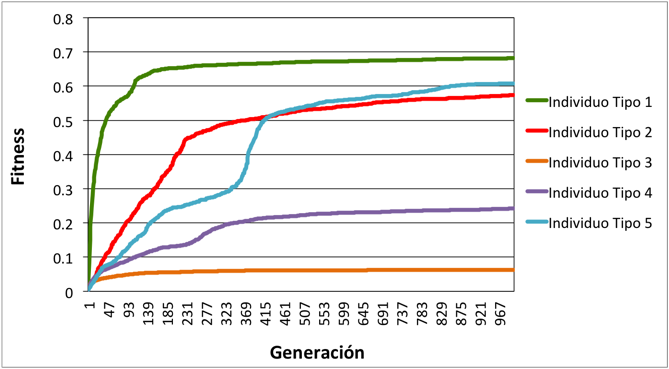
\includegraphics[width=0.72\linewidth]{resultados_001.png}} 
  \caption{Evoluci\'on del \textit{fitness} seg\'un tipo de individuos}%
  \label{fig:resultados_fitness} %
\end{figure}

\subsection{Velocidad seg\'un tipo de individuos}
Seguidamente, se muestra para cada individuo, su velocidad instant\'anea a lo largo del tiempo.
\begin{figure}[H]%
  \centering
  \frame{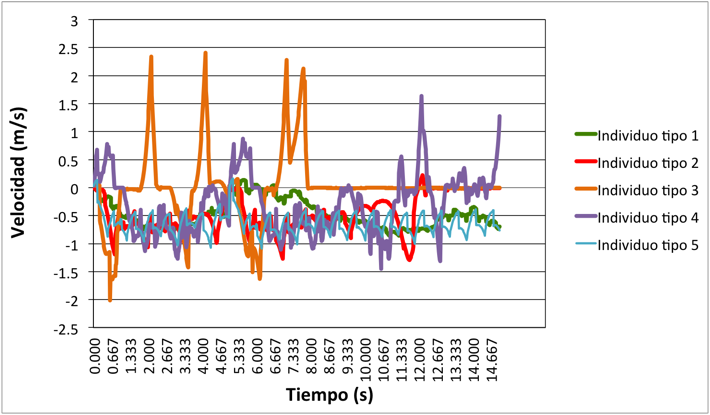
\includegraphics[width=0.72\linewidth]{resultados_003.png}} 
  \caption{Velocidad seg\'un tipo de individuos}%
  \label{fig:resultados_velocidad} %
\end{figure}
\noindent Como puede observarse en el caso de los individuos 3 y 4 (Fourier de orden 2 y 9, respectivamente), se producen picos altos y pronunciados en la velocidad. Eso repercute en que la velocidad media no sea 1.3 $\frac{m}{s}$ (que es la velocidad objetivo), y ergo, en el m\'odulo de velocidad del \textit{fitness} (provocando que \'este sea m\'as bajo).\\
%En el caso de los individuos 1 y 2, la velocidad instant\'anea oscila de forma suave. 
En el individuo de tipo 1, tambi\'en se producen picos un poco menos pronunciados, pero luego de los 10 segundos, no se registra ninguna velocidad. Eso sucede porque el humanoide queda suspendido cuando intenta caer hacia atr\'as.\\
La velocidad del individuo de tipo 2 oscila de forma irregular, pero no tiene picos muy elevados.\\ 
Por \'ultimo, en el individuo de tipo 5, la velocidad oscila de forma c\'iclica, continuada y armoniosa (no hay picos altos).

\subsection{Altura seg\'un tipo de individuos}
Como puede identificarse en la Figura \ref{fig:resultados_altura}, la altura de los individuos es otra caracter\'istica para diferenciarlos en su rendimiento.
\begin{figure}[H]%
  \centering
  \frame{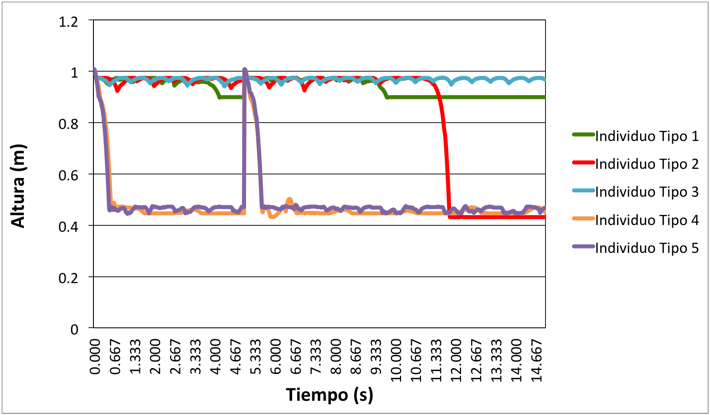
\includegraphics[width=0.72\linewidth]{resultados_002.png}} 
  \caption{Altura (posici\'on de la pelvis) seg\'un tipo de individuos}%
  \label{fig:resultados_altura} %
\end{figure}
\noindent En efecto, los individuos de tipo 3 y 4 (que utilizan actuadores de Fourier de orden 2 y 9, respectivamente), son los que caen de forma m\'as abrupta, y aunque intentan levantarse, vuelven a caer con la misma intensidad. \\
A su vez, el individuo de tipo 1 (actuador Gen\'erico sin funci\'on partida) mantiene su altura, hasta que a los 10 segundos queda suspendido a una altura levemente menor. Esto ocurre porque se cae para atr\'as, y las limitaciones de la cadera impiden que caiga. El individuo de tipo 2, con actuadores gen\'ericos y funci\'on partida, logra mantener la altura, hasta que cae hacia adelante, en cuclillas. Considerando que cuando cae no vuelve a levantarse (ya que en ese movimiento suelen emplearse los brazos y manos), tiene un comportamiento similar a una caminata real. \\
En lo que respecta al individuo de tipo 5, que utiliza como actuadores la funci\'on coseno doble frecuencia, mantiene su altura de forma constante, pero con oscilaciones leves y continuadas en el tiempo. De los cinco, es el que da mayor cantidad de pasos.


\subsection{Comparaci\'on de tipo de individuos}
En base a lo visto anteriormente, queda claro que los actuadores de Fourier no dieron buenos resultados tanto en fitness, como en altura y velocidad.\\
Por otra parte, es necesario incluir la funci\'on partida (es decir, separar a la caminata en un ``primer paso", y el ciclo), ya que si bien su ausencia puede originar \textit{fitness} m\'as altos, genera inestabilidad a los pocos segundos (como en el individuo de tipo 1).\\
El individuo de tipo 5 logra un movimiento c\'iclico y repetitvo, que deriva en una caminata \textit{ad infinitum}, pero con el costo de que sea ``rob\'otica" (muy parecida a lo visto con un \textit{passive walker}). 

\subsection{Video}
Para una mejor visualizaci\'on de los distintos individuos obtenidos, y de su evoluci\'on a lo largo de las generaciones del algoritmo gen\'etico, se acompa\~na video.\\
\textbf{Ac\'a va el link del video}


%----------------------------------------------------------------------------------------
%	SECTION 8 - CONCLUSIONES
%----------------------------------------------------------------------------------------

\section{Conclusiones}
El objetivo principal de este proyecto fue lograr producir la simulaci\'on y animaci\'on biomec\'anica de la caminata de un humano virtual. Para eso, se eligi\'o el motor f\'isico \textit{Bullet Physics}, lo que requiri\'o no solo aprender sobre su funcionamiento y los m\'etodos f\'isicos implementados, sino tambi\'en realizar pruebas para verificar qu\'e tan pr\'oximos eran el modelo fisico-matem\'atico ideado y el utilizado por Bullet.\\ % , en temas de coeficiente de fricci\'on y restituci\'on.\\
%Luego, se model\'o al humanoide como un conjunto de segmentos (cuerpos r\'igidos) unidos por articulaciones. Adem\'as, para desplazar al b\'ipedo y lograr la caminata, se aplicaron torques en cada uno de los segmentos (o actuadores),y otras funciones complementarias como funci\'on partida y fase sincronizada.\\
Una vez modelado el humanoide, se implementaron individuos con diferentes caracter\'isticas (en especial, actuadores), para facilitar la comparaci\'on. En la secci\'on \ref{resultados} se verifica que las funciones utilizadas en los actuadores son decisivas para lograr una caminata.\\
Los actuadores que mejores resultados dieron, fueron aquellos en donde se empleaba dos frecuencias $\omega$ en vez de una.\\
Lo ocurrido con el individuo de tipo 1 (gen\'erico y sin funci\'on partida), que es el que tiene un \textit{fitness} m\'as alto, aunque no produce una caminata acorde, posiblemente se deba a que el tiempo de simulaci\'on empleado en el algoritmo gen\'etico, fuera corto.\\
Se comprob\'o que los individuos con actuadores gen\'erico y coseno doble frecuencia son los que mejor caminan, manteniendo su altura por m\'as tiempo y con \textit{fitness} m\'as alto. Sin embargo, son caminatas muy distintas: la del primero resulta ser m\'as natural, pero se cae m\'as r\'apido; mientras que la del segundo es m\'as ``rob\'otica" (ya que parece un \textit{passive walker}), pero m\'as estable (no se cae nunca ni se queda quieto).\\
La funci\'on de fitness que se plantea (con sus m\'odulos) indica propiedades ideales para una caminata, pero que no implican realismo en la misma. Y entonces dos individuos con \textit{fitness} parecidos dieron como fruto caminatas muy distintas.\\
Si hay que elegir como mejor a uno de los dos, habr\'ia que decidir entre realismo (el humanoide se cae, pero es m\'as natural), y estabilidad (no se cae, pero parece un \textit{passive walker}).\\
Entre los trabajos a futuro para integrar a este proyecto, se encuentran lograr que la caminata se produzca en 3 dimensiones; y analizar el comportamiento de varios humanoides chocando e  interactuando entre s\'i.\\
Se puede concluir que, la caminata de una persona, algo que parece simple y sencillo, muestra su verdadera complejidad cuando debe ser simulada por medio de actuadores aplicados a un conjunto de segmentos interconectados.


%----------------------------------------------------------------------------------------
%	BIBLIOGRAPHY
%----------------------------------------------------------------------------------------

\begin{thebibliography}{1}
\bibitem{Wojtyra}
Marek Wojtyra, \emph{Multibody Simulation Model of Human Walking - Warsaw University of Technology, 2003}
\bibitem{flexibleMuscle}
Thomas Geijtenbeek, Michiel van de Panne y A. Frank van der Stappen, \emph{Flexible Muscle-Based Locomotion for Bipedal Creatures, 2013 }
\bibitem{Cuadrupedo}
Kevin Kenny, M\'aximo Videla y Axel Wassington, \emph{Proyecto Final para la obtenci\'on del t\'itulo Ingeniero en Inform\'atica: Simulaci\'on y animaci\'on de un cuadr\'upedo virtual - ITBA, 2014}
\bibitem{wikiPhysicsEngine} Wikipedia: $https://es.wikipedia.org/wiki/Physics\_engine$
\bibitem{Comparissons}
Andreas Gerndt y otros, \emph{An Evaluation of Open Source Physics Engines for Use in Virtual Reality Assembly Simulations. Fecha de publicaci\'on: 2012}
\bibitem{Comparissons2}
Tom Erez y otros, \emph{Simulation Tools for Model-Based Robotics: Comparison of \textit{Bullet}, Havok, MuJoCo, ODE and PhysX}
\bibitem{LinkBullet} Sitio web de Bullet Physics: $http://www.bulletphysics.org/$
\bibitem{Catto}
Erin Catto, \emph{Iterative Dynamic with Temporal Coherence. Fecha de publicaci\'on: 2005}
\bibitem{LinkGaLib} Sitio web de GaLib: $http://lancet.mit.edu/ga/$
\bibitem{biomechanics}$http://www.exrx.net/Kinesiology/Segments.html$

\end{thebibliography}

%----------------------------------------------------------------------------------------


\end{document}
